\documentclass[12pt,letterpaper]{article}
\usepackage{graphicx,textcomp}
\usepackage{natbib}
\usepackage{setspace}
\usepackage{fullpage}
\usepackage{color}
\usepackage[reqno]{amsmath}
\usepackage{amsthm}
\usepackage{fancyvrb}
\usepackage{amssymb,enumerate}
\usepackage[all]{xy}
\usepackage{endnotes}
\usepackage{lscape}
\newtheorem{com}{Comment}
\usepackage{float}
\usepackage{hyperref}
\newtheorem{lem} {Lemma}
\newtheorem{prop}{Proposition}
\newtheorem{thm}{Theorem}
\newtheorem{defn}{Definition}
\newtheorem{cor}{Corollary}
\newtheorem{obs}{Observation}
\usepackage[compact]{titlesec}
\usepackage{dcolumn}
\usepackage{tikz}
\usetikzlibrary{arrows}
\usepackage{multirow}
\usepackage{xcolor}
\newcolumntype{.}{D{.}{.}{-1}}
\newcolumntype{d}[1]{D{.}{.}{#1}}
\definecolor{light-gray}{gray}{0.65}
\usepackage{url}
\usepackage{listings}
\usepackage{color}
\usepackage{adjustbox}
\usepackage{caption}
\captionsetup{justification=centering}

\definecolor{codegreen}{rgb}{0,0.6,0}
\definecolor{codegray}{rgb}{0.5,0.5,0.5}
\definecolor{codepurple}{rgb}{0.58,0,0.82}
\definecolor{backcolour}{rgb}{0.95,0.95,0.92}

\lstdefinestyle{mystyle}{
	backgroundcolor=\color{backcolour},   
	commentstyle=\color{codegreen},
	keywordstyle=\color{magenta},
	numberstyle=\tiny\color{codegray},
	stringstyle=\color{codepurple},
	basicstyle=\footnotesize,
	breakatwhitespace=false,         
	breaklines=true,                 
	captionpos=b,                    
	keepspaces=true,                 
	numbers=left,                    
	numbersep=5pt,                  
	showspaces=false,                
	showstringspaces=false,
	showtabs=false,                  
	tabsize=2
}
\lstset{style=mystyle}
\newcommand{\Sref}[1]{Section~\ref{#1}}
\newtheorem{hyp}{Hypothesis}

\title{Replication Project - Stats II}
\date{31 April, 2024}
\author{Sara Cid}

\begin{document}
	
\maketitle

\section*{Introduction} 
\vspace{.25cm}

\noindent This paper presents the results of replicating the main figures and tables in  
\href{doi:10.1017/S0003055423000369}{Tavits, M., Schleiter, P., Homola, J., \& Ward, D. (2024). ``Fathers’Leave Reduces Sexist Attitudes"}. 
The replication materials were found in the Harvard Dataverse,
\href{https://dataverse.harvard.edu/dataset.xhtml?persistentId=doi:10.7910/DVN/4DUB7X}{\textcolor{blue}{here}}.

The article looks at the effect of paternity leave policies on sexist attitudes in society. The authors exploit the introduction of a three week extension in “daddy leave" in Estonia using a design similar to Regression Discontinuity, and applying surveys to couples whose children's births are due right after vs. right before the new length of the leave took effect. The study also controls for several variables like education, socio-economic status, gender and age to isolate the effects of daddy leave over three different attitude scales. 

The scales are the Socio-Economic Scale (here, the survey has items like agreement/disagreement that “a preschool child is likely to suffer if his or her mother works"), the Political Scale (asking respondents, for instance, about their agreement/disagree-ment that “men make better political leaders than women do"), and the Positive Action Scale (asking respondents about their agreement/ disagreement with, for instance, requiring “political parties to reserve some space on their lists of candidates for women, even if they have to exclude some men"). 

The paper presents causal evidence that the introduction of paternity leave policies is associated with a significant reduction in sexist attitudes among both men and women who are soon-to-be parents, but not among society in general (direct exposure has an effect on attitudes, but indirect or informational exposure does not). For the Socio-Economic equality Scale, the effect of the policy is the most sizable (it is comparable to the effect of being female). In addition, evidence of a positive impact on attitudes in the political domain are also found, but not for the Positive Action Scale. 

\newpage
\vspace{.5cm}
\section*{Replicated Figures and Tables} 
\vspace{.25cm}

\noindent The figures and tables from the main text of the article were replicated. The replication files found on the Harvard Dataverse were excellent, and the R code produced the figures with ease. No problems were found with the code or models. The main text includes one table and three figures. Each of these are presented and briefly explained below. 

 First, the paper presents Table 1, which includes manipulation checks. These checks show that the parents are aware of the reform. The researchers asked respondents three questions for this: how long they thought a father was entitled to take (Entitlement), how long they thought fathers take on average (Average), and how much leave they are planning to take with their new baby (Uptake). As the Table shows, the responses are as expected according to the group participants belong to (treatment or control). 

\begin{table}[!htbp] \centering   \caption{Manipulation Checks}   \label{} \begin{tabular}{@{\extracolsep{5pt}} D{.}{.}{-3} D{.}{.}{-3} D{.}{.}{-3} D{.}{.}{-3} D{.}{.}{-3} } \\[-1.8ex]\hline \hline \\[-1.8ex] \multicolumn{1}{c}{Measure} & \multicolumn{1}{c}{PreReform} & \multicolumn{1}{c}{PostReform} & \multicolumn{1}{c}{Difference} & \multicolumn{1}{c}{N} \\ \hline \\[-1.8ex] \multicolumn{1}{c}{Entitlement} & \multicolumn{1}{c}{13.26} & \multicolumn{1}{c}{29.48} & \multicolumn{1}{c}{16.22 (p \textless  0.01)} & 1,359 \\ \multicolumn{1}{c}{Average Use} & \multicolumn{1}{c}{9.67} & \multicolumn{1}{c}{18.50} & \multicolumn{1}{c}{8.82 (p \textless  0.01)} & 1,357 \\ \multicolumn{1}{c}{Uptake (fathers)} & \multicolumn{1}{c}{15.56} & \multicolumn{1}{c}{27.03} & \multicolumn{1}{c}{11.47 (p \textless  0.01)} & 610 \\ \multicolumn{1}{c}{Uptake (mothers)} & \multicolumn{1}{c}{334.89} & \multicolumn{1}{c}{341.00} & \multicolumn{1}{c}{6.11 (p = 0.75)} & 712 \\ \hline \\[-1.8ex] \end{tabular} \end{table} 

\newpage
\noindent Next, Figure 1 presents the effects of the policy change on the three scales, for soon-to-be parents, who received direct exposure to the policy. This Figure shows that the policy significantly increased attitudinal support for for gender equality in the social and economic spheres (the very top of the Figure), as well as causing a moderate increase in the Political Scale. The estimates for the effects on the Positive Action Scale, however, are a lot smaller and not statistically significant. 

\begin{figure}[H]
	\centering
	\caption{Effect of Fathers’ Leave Reform on Gender-Equal Attitudes, Study 1 (Direct Exposure)}
	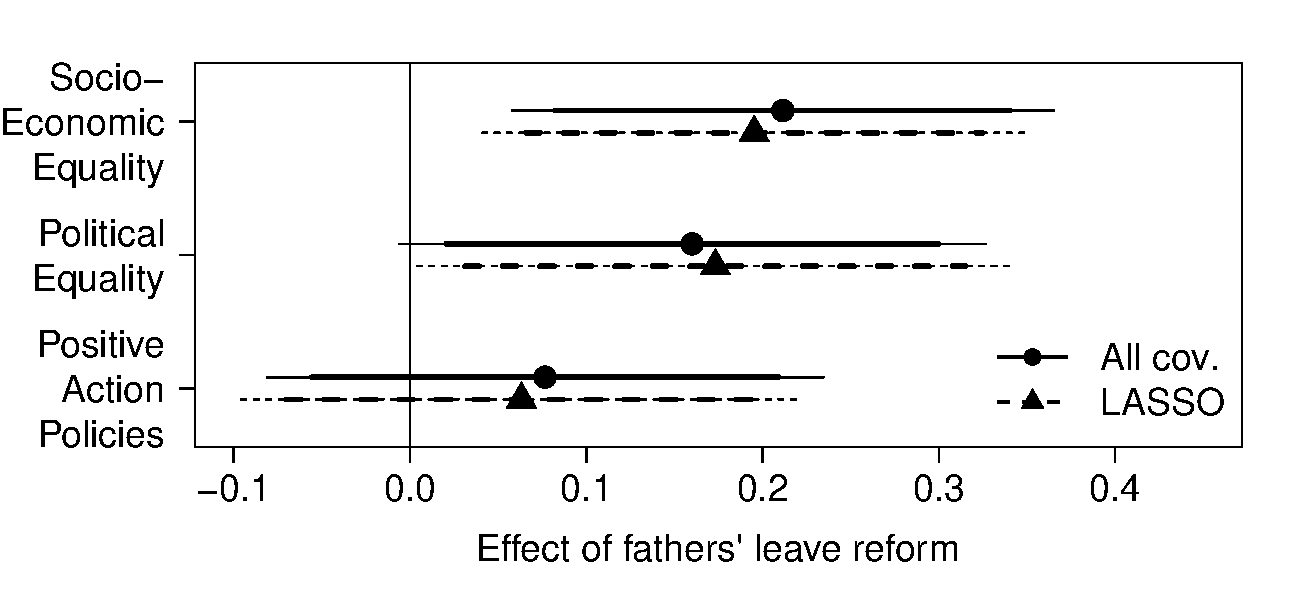
\includegraphics[width=0.8\textwidth]{Fig1}
	\label{fig:my_label}
\end{figure}

\newpage
\noindent Figure 2 presents the results of an analysis split by sex, which reveals that the increase for support for gender equality in the Socio-Economic and Political Scales that the policy causes is similar for fathers and mothers, but the differences for the Positive Action Scale are striking. For mothers, the effect of the reform is positive, large, and statistically significant, while the authors find no statistically significant increase for fathers. 

\begin{figure}[H]
	\centering
	\caption{Effect of Fathers’ Leave Reform on Gender-Equal Attitudes for Mothers and Fathers, Study 1(Direct Exposure)}
	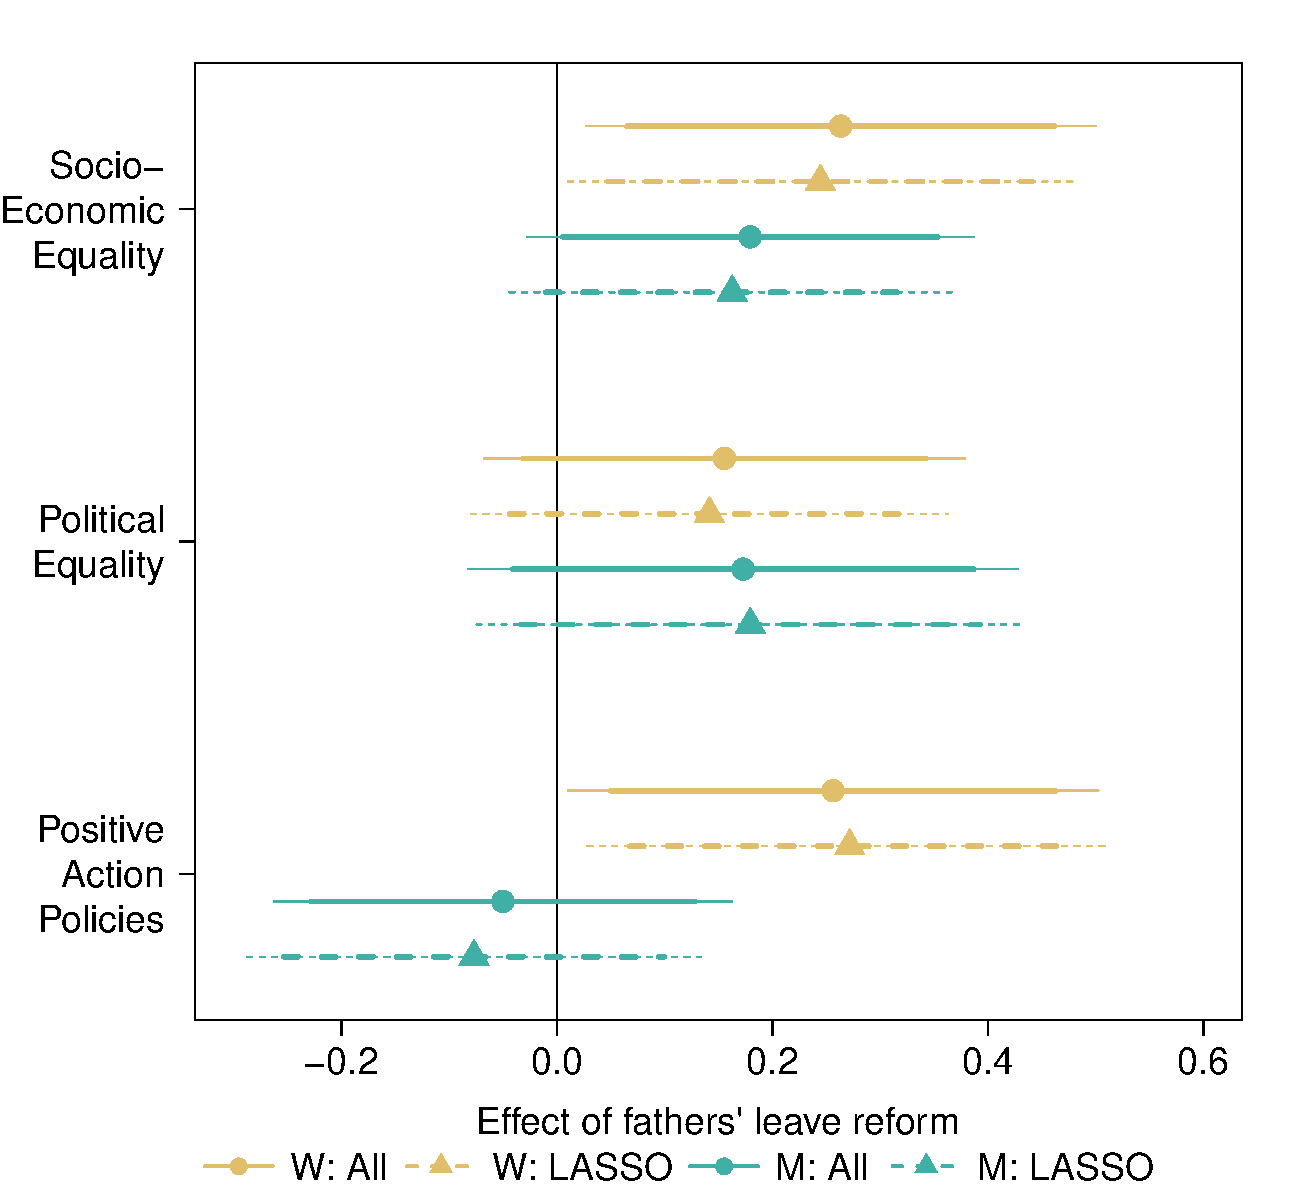
\includegraphics[width=0.8\textwidth]{Fig2}
	\label{fig:my_label}
\end{figure}

\newpage
\noindent Figure 3 presents the effects of the policy change on the three scales, for the general public, who received what the authors call indirect or informational exposure to the policy. This Figure shows that the policy had no effect on attitudes towards gender equality in this population. Thus, the authors conclude that informational exposure is a less effective means for increasing attitudinal support for gender equality. 

\begin{figure}[H]
	\centering
	\caption{Effect of Information about the Reform on Gender-Equal Attitudes, Study 2 (Indirect Exposure)}
	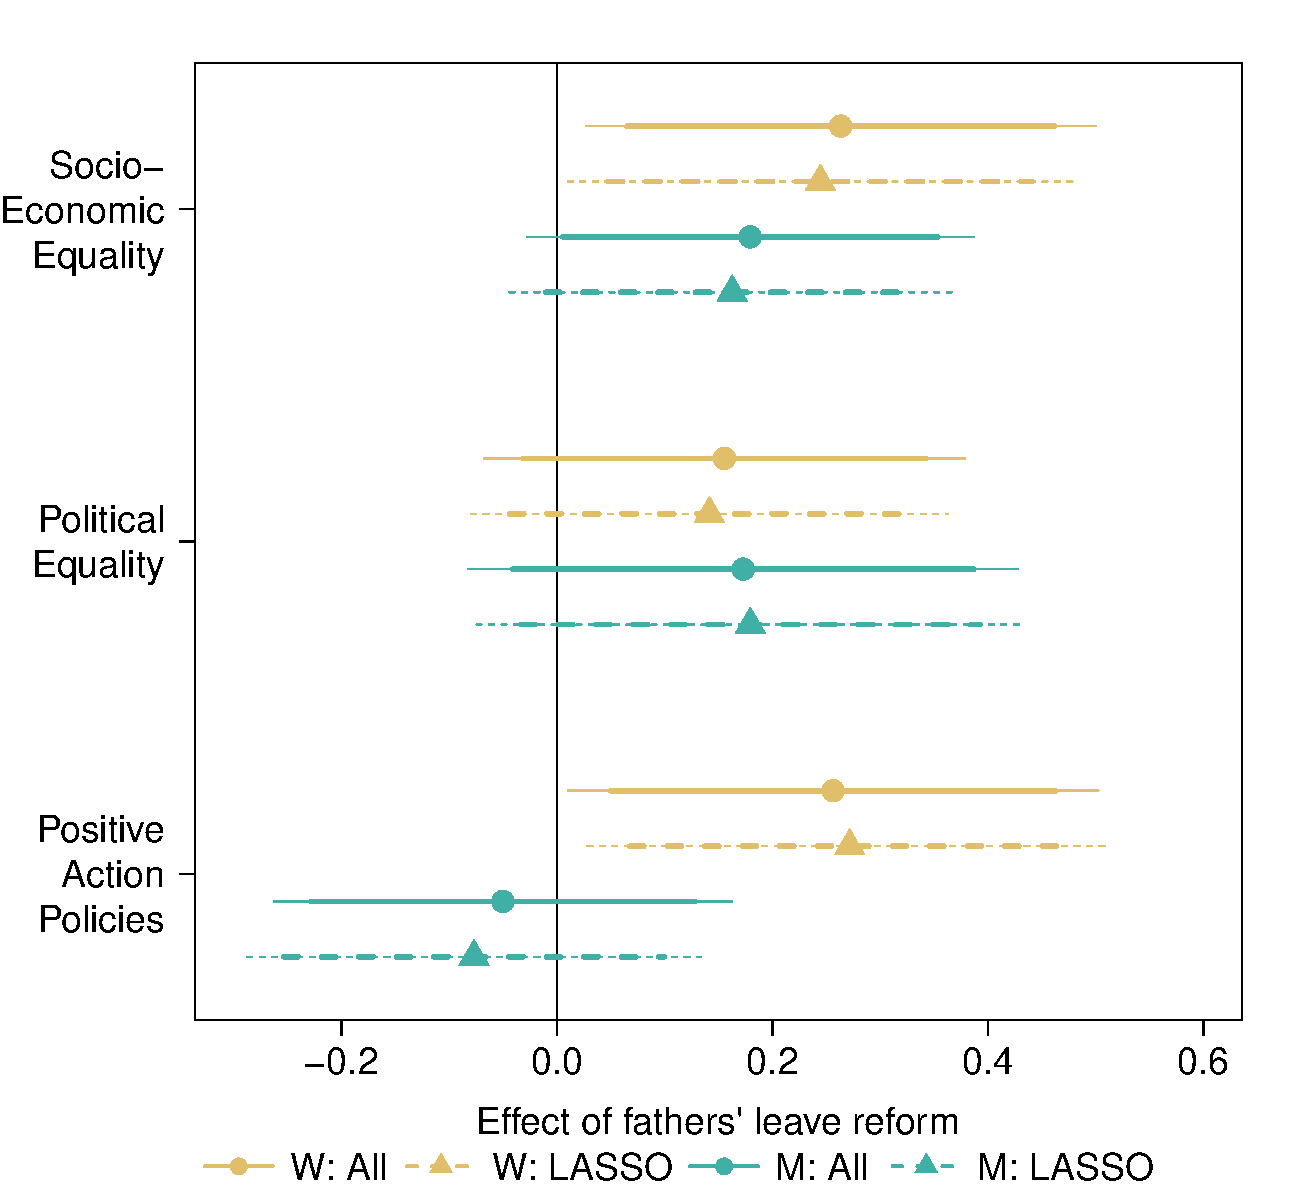
\includegraphics[width=0.8\textwidth]{Fig2}
	\label{fig:my_label}
\end{figure}

\newpage
\section*{Contribution} 
\vspace{.25cm}
\noindent 

\noindent To introduce a twist to the article, an examination of how other variables may add to the models and interact with the daddy leave policy was carried out. While the authors present the results of the analysis split by gender (this is what Figure 2 describes), and while they do include controls, as well as interactions in their Lasso models (those that were automatically selected by the Lasso method), this is not the main focus on the study. Therefore, as an addition to the paper, I explore how different variables in the authors' dataset can affect the outcomes directly, as well as interact with the daddy leave reform variable to affect the outcomes. 

\vspace{0.35cm}
\noindent Seven variables were selected. In what remains of this paper, the reasoning behind the inclusion of these variables (both as controls and interacting variables) is discussed, and the results of including them on their own and interacting with the main predictor are presented. 

\begin{enumerate}
	\item \textbf{Gender}: 
	
	\noindent Gender might both affect the outcomes directly or mediate the effects of the policy for plenty of reasons. First, it would probably be expected for women to have more favorable attitudes towards gender equality, so we would expect the relationship between female and the scales to be positive. For the interaction of gender with the policy, on the other hand, since the leave policy affects fathers directly, and mothers only indirectly through their partners' choices, perhaps the effect of the policy on gender equality attitudes would be larger for dads. 
	
	\noindent As Figure 4 shows, women have more favorable attitudes on all the scales, as it would be expected, and the coefficient estimate for gender is statistically significant in all the models. When looking at the interactive effects, the slopes of the regression lines for the Socio-Economic and Political Scales show that the reasoning presented above could be correct, as the effect of the reform seems more pronounced for fathers than for mothers. This is the opposite in the Positive Action scale, however, where the slope for men is negative. The estimated coefficient for the interaction term is, however, not statistically significant for any of the models. 
	
	\begin{figure}[H]
		\centering
		\caption{Predicted Effects of Reform with added Gender Variable and Interaction Across Scales}
		\vspace{-1cm}
		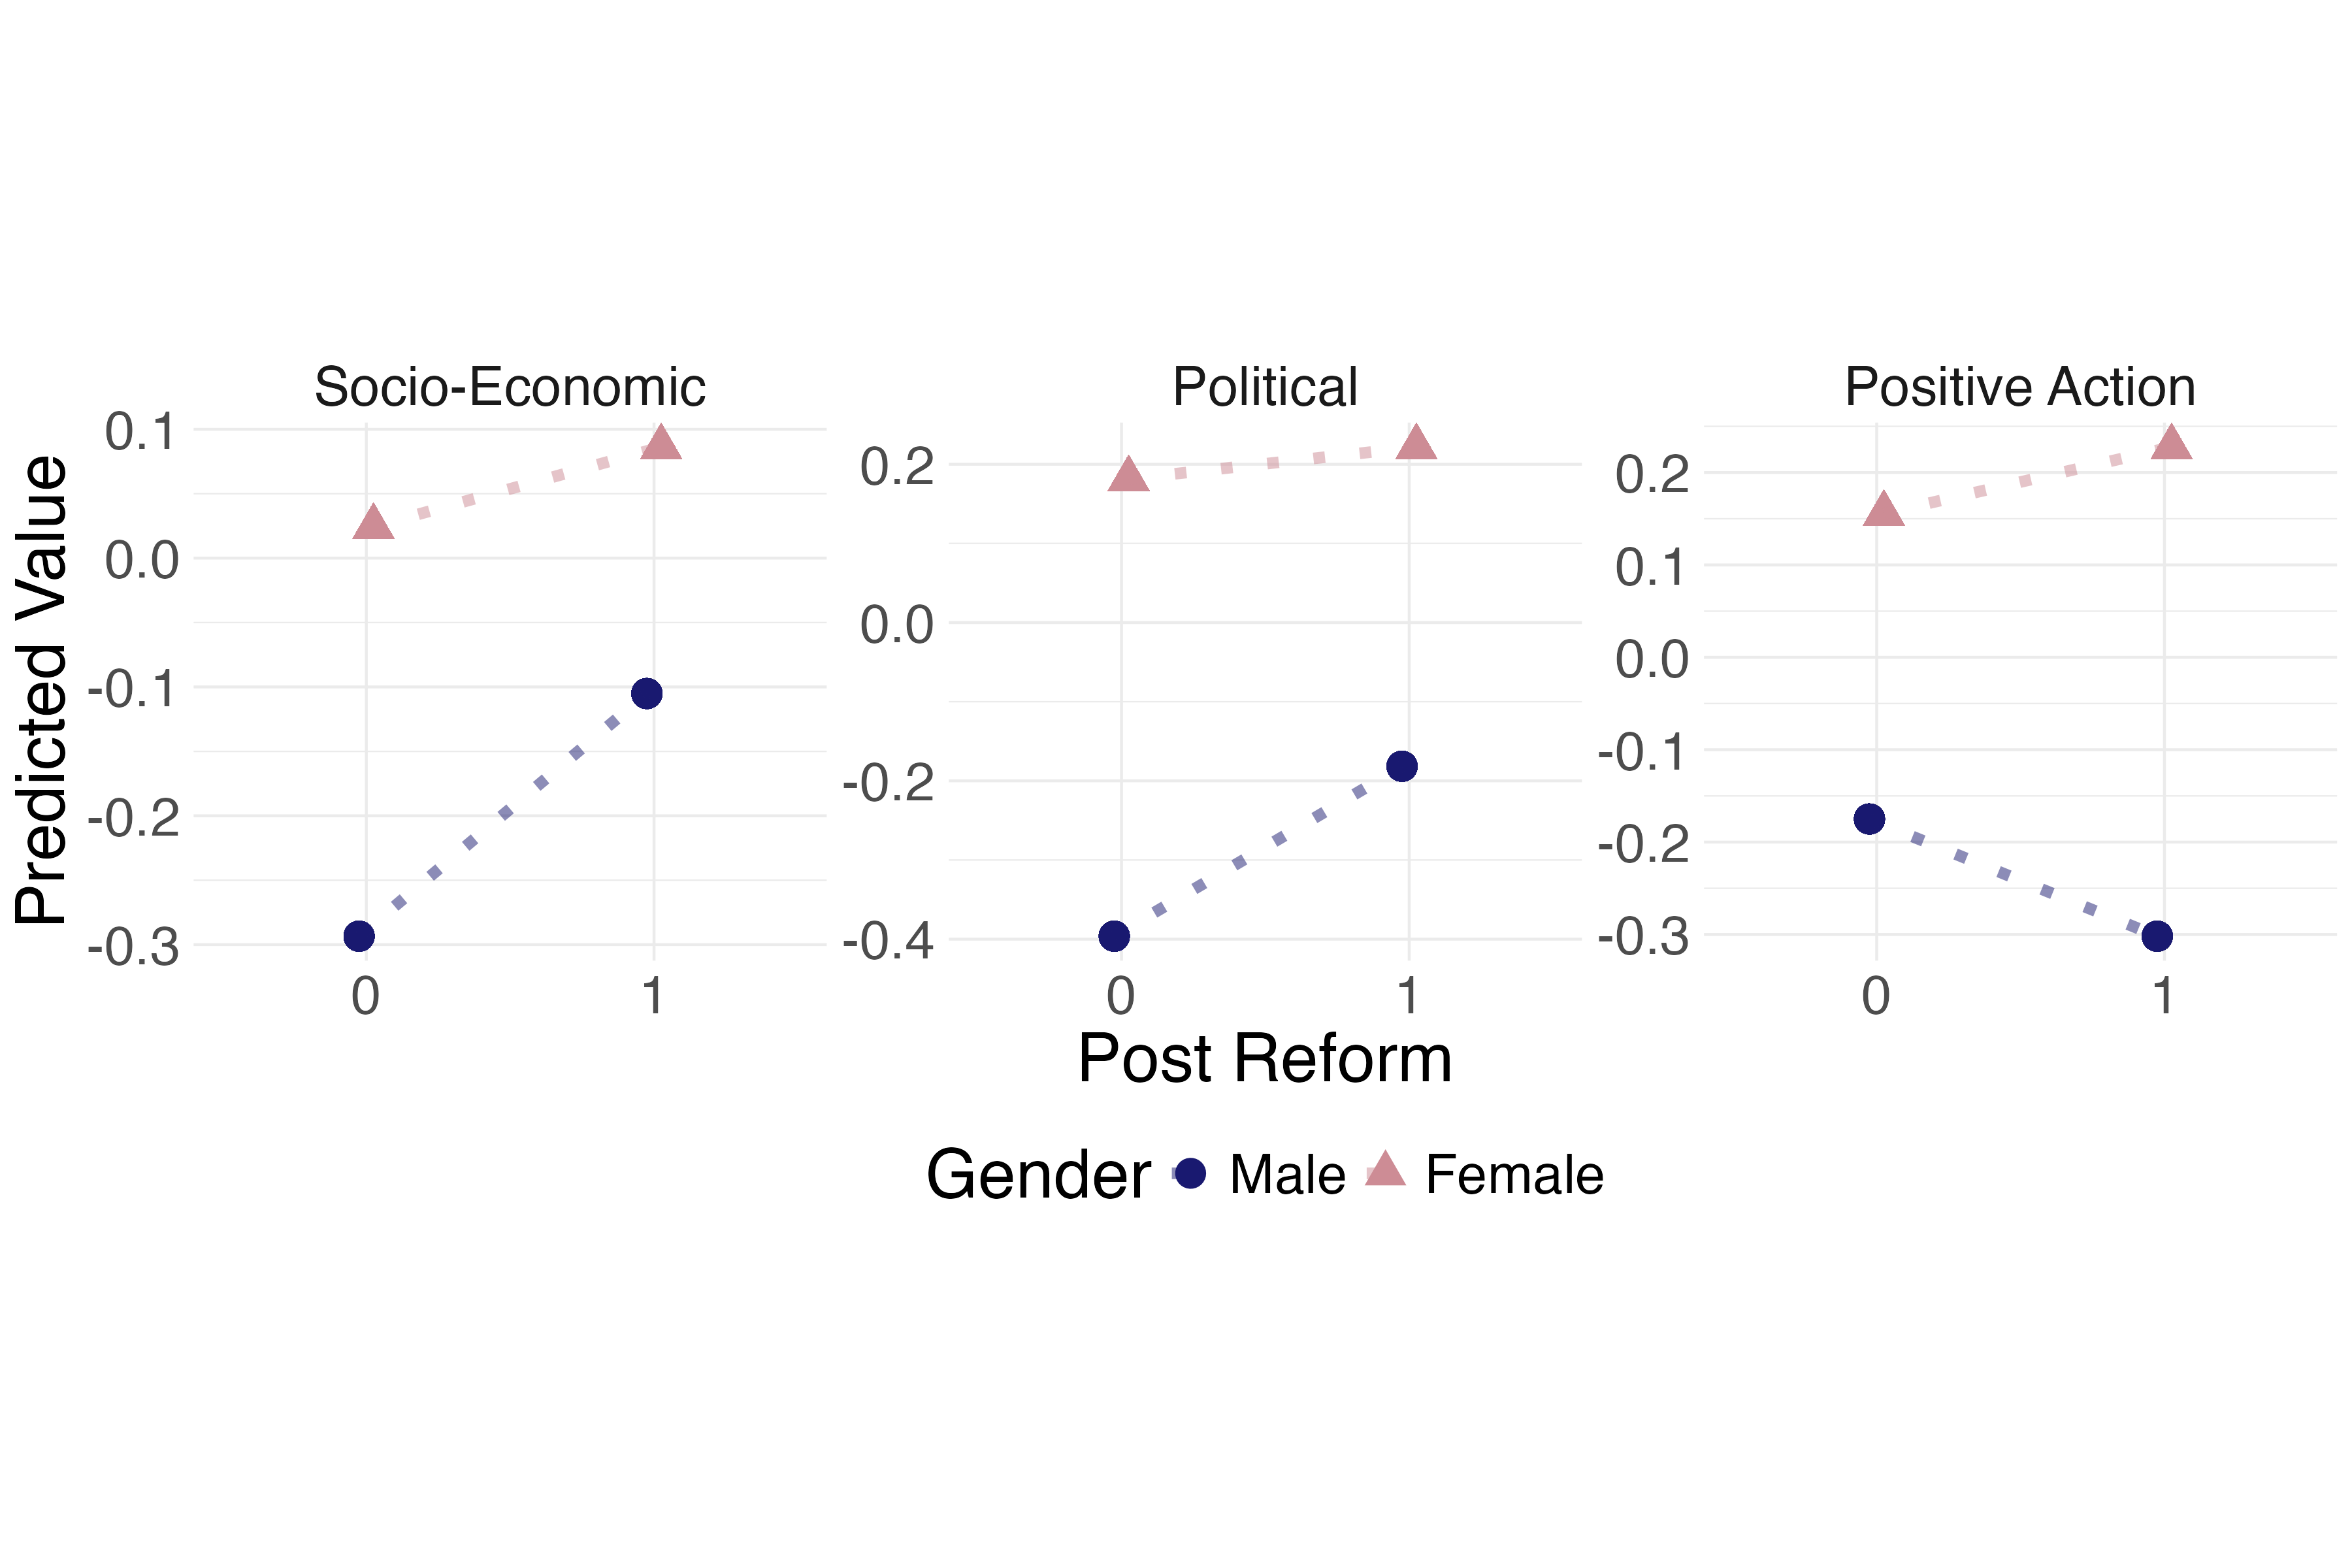
\includegraphics[width=0.9\textwidth]{gender_plot}
		\label{fig:gender_plot}
	\end{figure}
	
	\begin{table}[H] \centering   \caption{Gender Models}   \label{} \begin{tabular}{@{\extracolsep{5pt}}lccc} \\[-1.8ex]\hline \hline \\[-1.8ex]  & \multicolumn{3}{c}{\textit{Dependent variable:}} \\ \cline{2-4} \\[-1.8ex] & SocEconScale & PolScale & PosActScale \\ \\[-1.8ex] & (1) & (2) & (3)\\ \hline \\[-1.8ex]  postReform1 & 0.188$^{*}$ & 0.215$^{**}$ & $-$0.127 \\   & (0.104) & (0.105) & (0.099) \\   & & & \\  female & 0.318$^{***}$ & 0.578$^{***}$ & 0.331$^{***}$ \\   & (0.119) & (0.120) & (0.113) \\   & & & \\  postReform1:female & $-$0.127 & $-$0.174 & 0.199 \\   & (0.148) & (0.149) & (0.140) \\   & & & \\  Constant & $-$0.293$^{***}$ & $-$0.396$^{***}$ & $-$0.175$^{**}$ \\   & (0.081) & (0.082) & (0.077) \\   & & & \\ \hline \\[-1.8ex] Observations & 800 & 799 & 799 \\ R$^{2}$ & 0.020 & 0.059 & 0.058 \\ Adjusted R$^{2}$ & 0.016 & 0.055 & 0.055 \\ Residual Std. Error & 0.989 (df = 796) & 0.998 (df = 795) & 0.940 (df = 795) \\ F Statistic & 5.330$^{***}$ (df = 3; 796) & 16.507$^{***}$ (df = 3; 795) & 16.461$^{***}$ (df = 3; 795) \\ \hline \hline \\[-1.8ex] \textit{Note:}  & \multicolumn{3}{r}{$^{*}$p$<$0.1; $^{**}$p$<$0.05; $^{***}$p$<$0.01} \\ \end{tabular} \end{table} 
	
	\newpage
	\item \textbf{University}: 
	
	\noindent First, we would expect people with more schooling and university education to exhibit higher baseline scores in the three Scales, as university-educated people typically show more progressive views (in good measure, for variables other than being university-educated per se, but that correlate with such educational attainment). Thus, we would expect the coefficient of the additional term of University to be positive. Moreover, university education may either make people amplify or show muted changes in attitudes towards gender equality due to the pre-existing progressive views that are typically associated with university, so the direction of the interaction effect could be unclear. 
	
	\noindent Figure 5 shows, first, that the baseline support for gender equality is indeed higher for university-educated people, except for the Positive Action Scale. For the models with the Positive Action Scale as an outcome, however, no results were statistically significant. The coefficients for University in the Socio-Economic and Political Scale models were all positive and statistically significant, though. Thus, as expected, people who went to University do have more support for gender equality to begin with. Secondly, with regard to the interactions, while the slopes vary per group (in the Socio-Economic model, it would seem like university-educated people muting changes is the case), no interaction term was found to be statistically significant. 
	
	\begin{figure}[H]
		\centering
		\caption{Predicted Effects of Reform with added University Education Variable and Interaction Across Scales}
		\vspace{-1cm}
		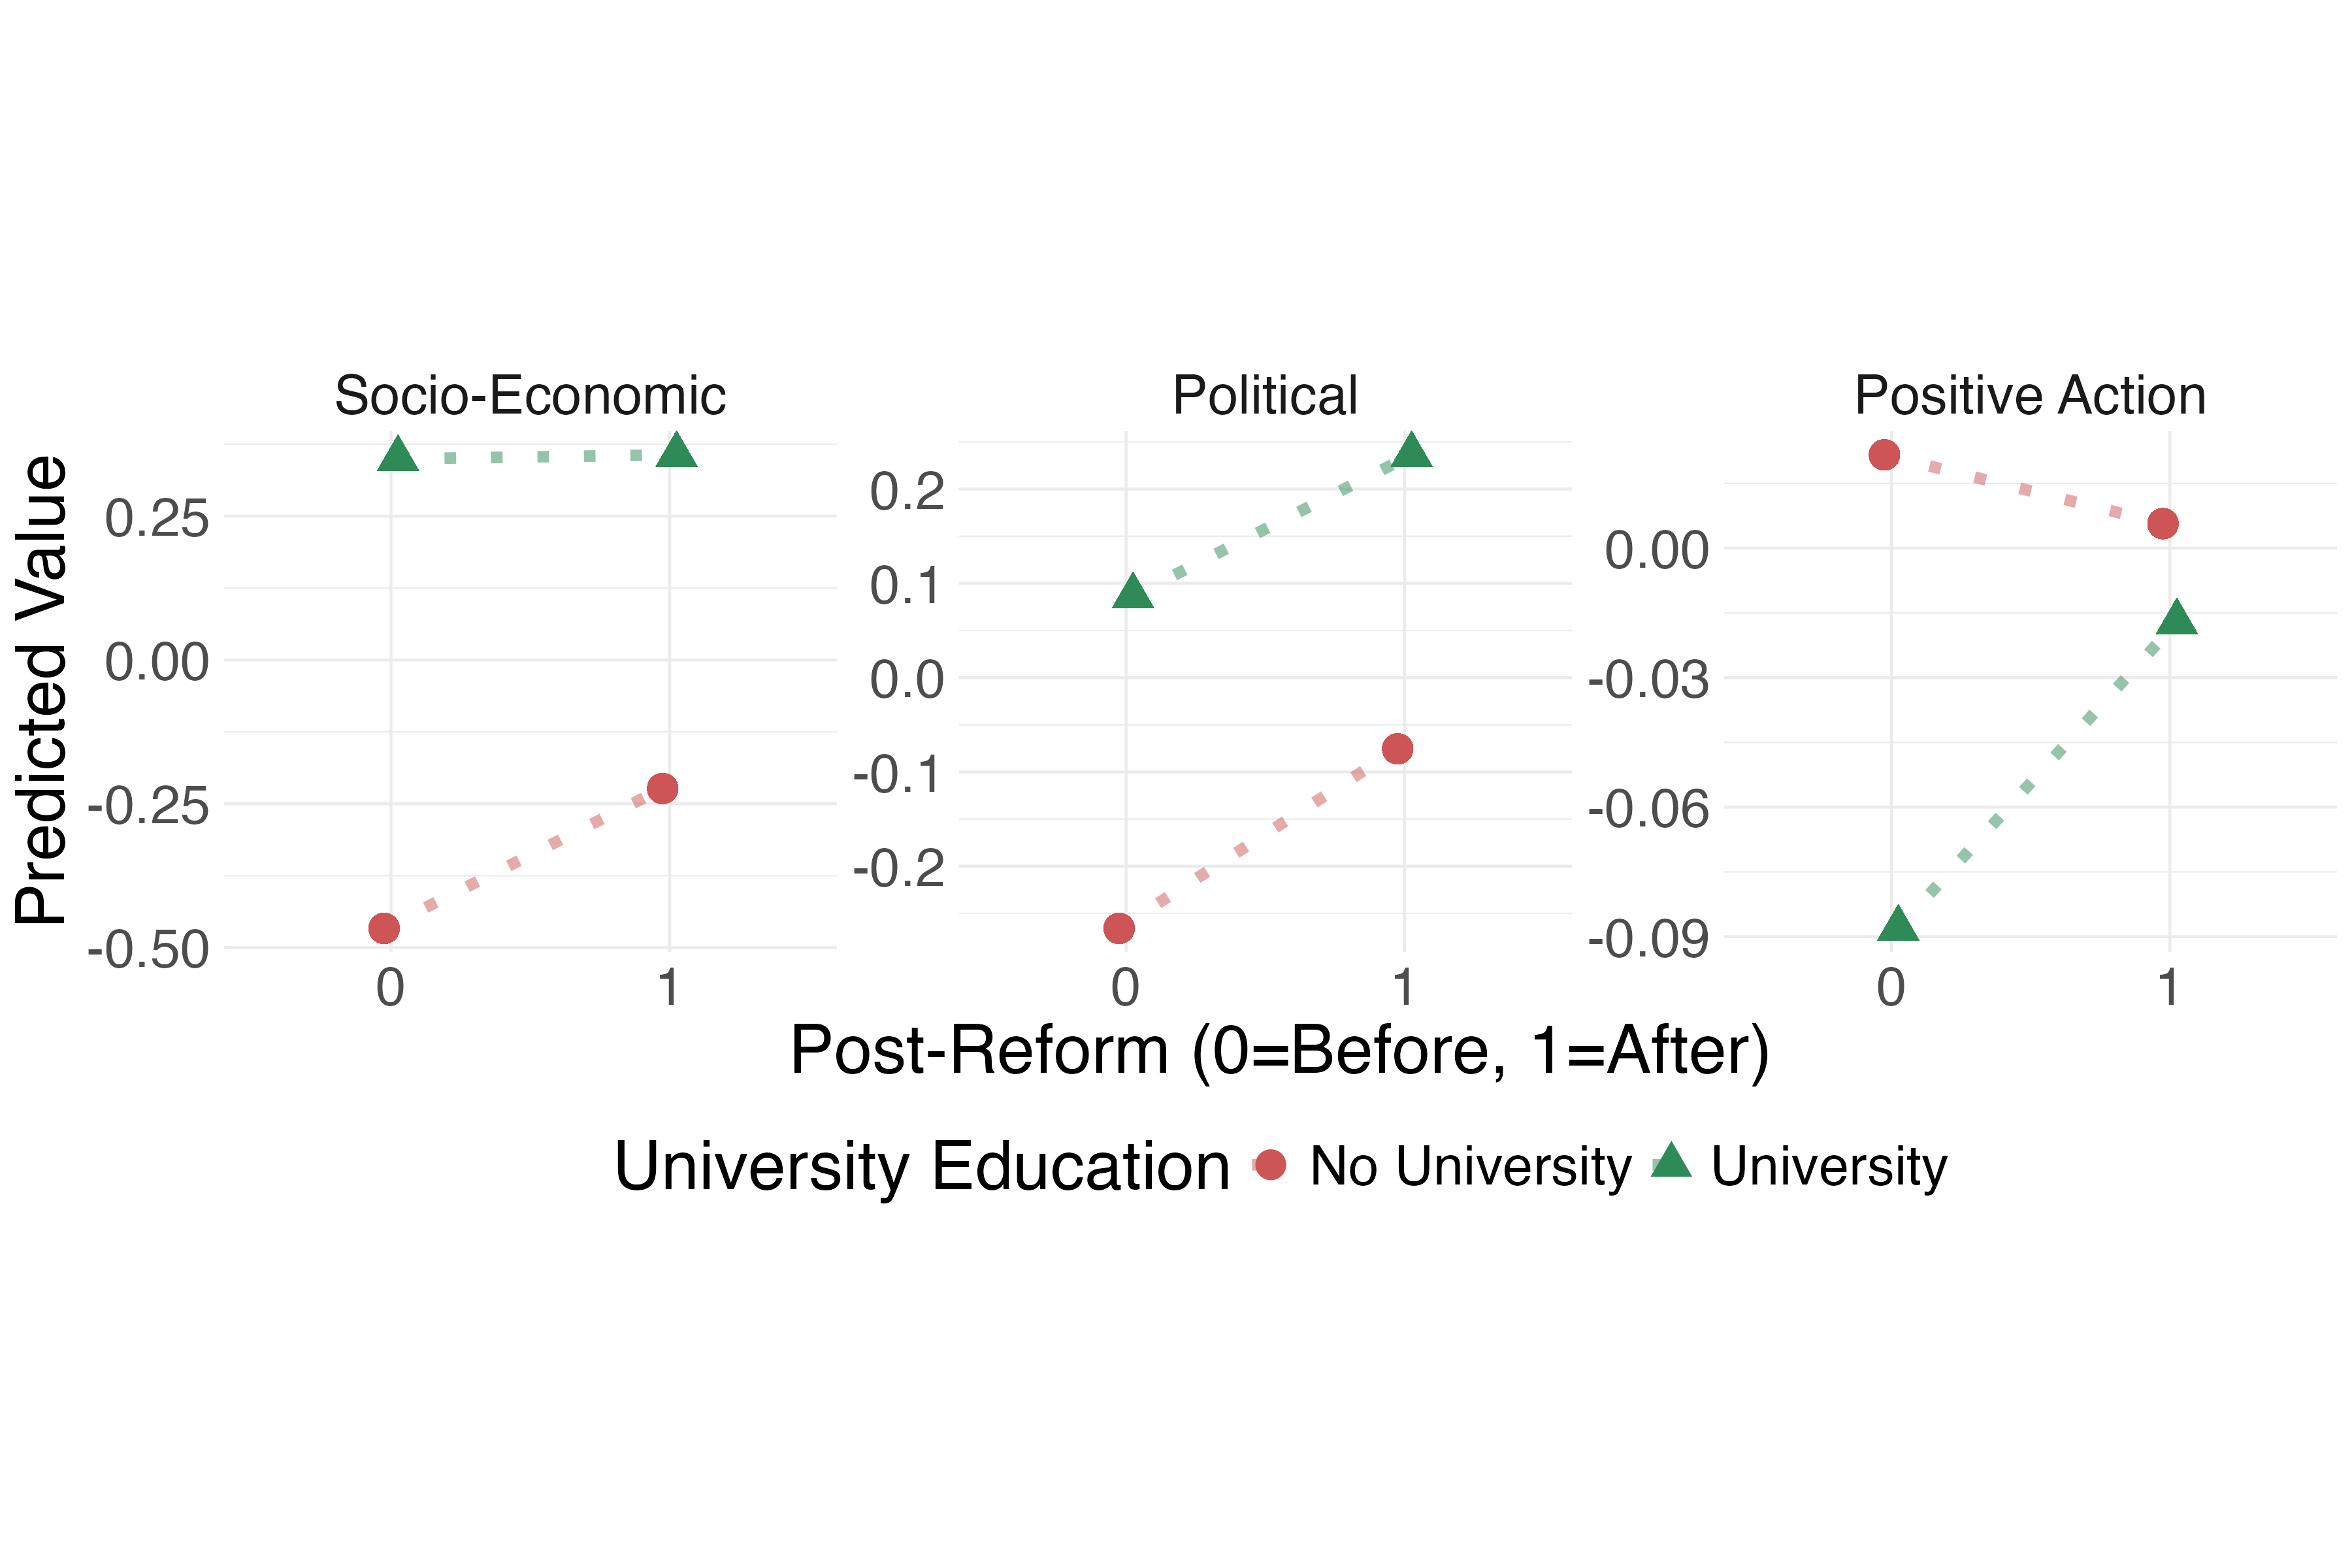
\includegraphics[width=0.9\textwidth]{univ_plot}
		\label{fig:univ_plot}
	\end{figure}
	
	\begin{table}[H] \centering   \caption{Education Models}   \label{} \begin{tabular}{@{\extracolsep{5pt}}lccc} \\[-1.8ex]\hline \hline \\[-1.8ex]  & \multicolumn{3}{c}{\textit{Dependent variable:}} \\ \cline{2-4} \\[-1.8ex] & SocEconScale & PolScale & PosActScale \\ \\[-1.8ex] & (1) & (2) & (3)\\ \hline \\[-1.8ex]  postReform1 & 0.243$^{***}$ & 0.190$^{**}$ & $-$0.016 \\   & (0.090) & (0.097) & (0.092) \\   & & & \\  edu\_uni & 0.817$^{***}$ & 0.353$^{***}$ & $-$0.110 \\   & (0.116) & (0.125) & (0.119) \\   & & & \\  postReform1:edu\_uni & $-$0.236$^{*}$ & $-$0.041 & 0.087 \\   & (0.143) & (0.154) & (0.147) \\   & & & \\  Constant & $-$0.467$^{***}$ & $-$0.266$^{***}$ & 0.022 \\   & (0.073) & (0.078) & (0.075) \\   & & & \\ \hline \\[-1.8ex] Observations & 800 & 799 & 799 \\ R$^{2}$ & 0.113 & 0.031 & 0.001 \\ Adjusted R$^{2}$ & 0.110 & 0.027 & $-$0.003 \\ Residual Std. Error & 0.941 (df = 796) & 1.013 (df = 795) & 0.968 (df = 795) \\ F Statistic & 33.859$^{***}$ (df = 3; 796) & 8.366$^{***}$ (df = 3; 795) & 0.327 (df = 3; 795) \\ \hline \hline \\[-1.8ex] \textit{Note:}  & \multicolumn{3}{r}{$^{*}$p$<$0.1; $^{**}$p$<$0.05; $^{***}$p$<$0.01} \\ \end{tabular} \end{table} 
	
	\newpage
	\item \textbf{Age}: 
	
	\noindent For age, we would expect younger individuals to have higher baseline scores on the gender equality Scales, as the older population tends to be more conservative, so the sign of the age coefficient should be negative. As for the interaction, the effect of daddy leave policy could vary by age, perhaps with more pronounced effects among older individuals, since they have been exposed to more traditional norms before. 
	
	\noindent As we see in Figure 6, the baseline support for gender equality does not in fact seem to be lower as age increases, since mature adults (30 to 35 years old) have the highest scores (except for the Positive Action Scale). Also, from Table 4 we see that the coefficient for the mature adults category is positive and statistically significant for the Socio-Economic Scale (where the reference category is "younger adults"), and so is the coefficient of the interaction term between mature adults and the reform. This last coefficient is negative, indicating that the effect of the policy for this age category is attenuated. 
	
	\begin{figure}[H]
		\centering
		\caption{Predicted Effects of Reform with added Age Group Variable and Interaction Across Scales}
		\vspace{-1cm}
		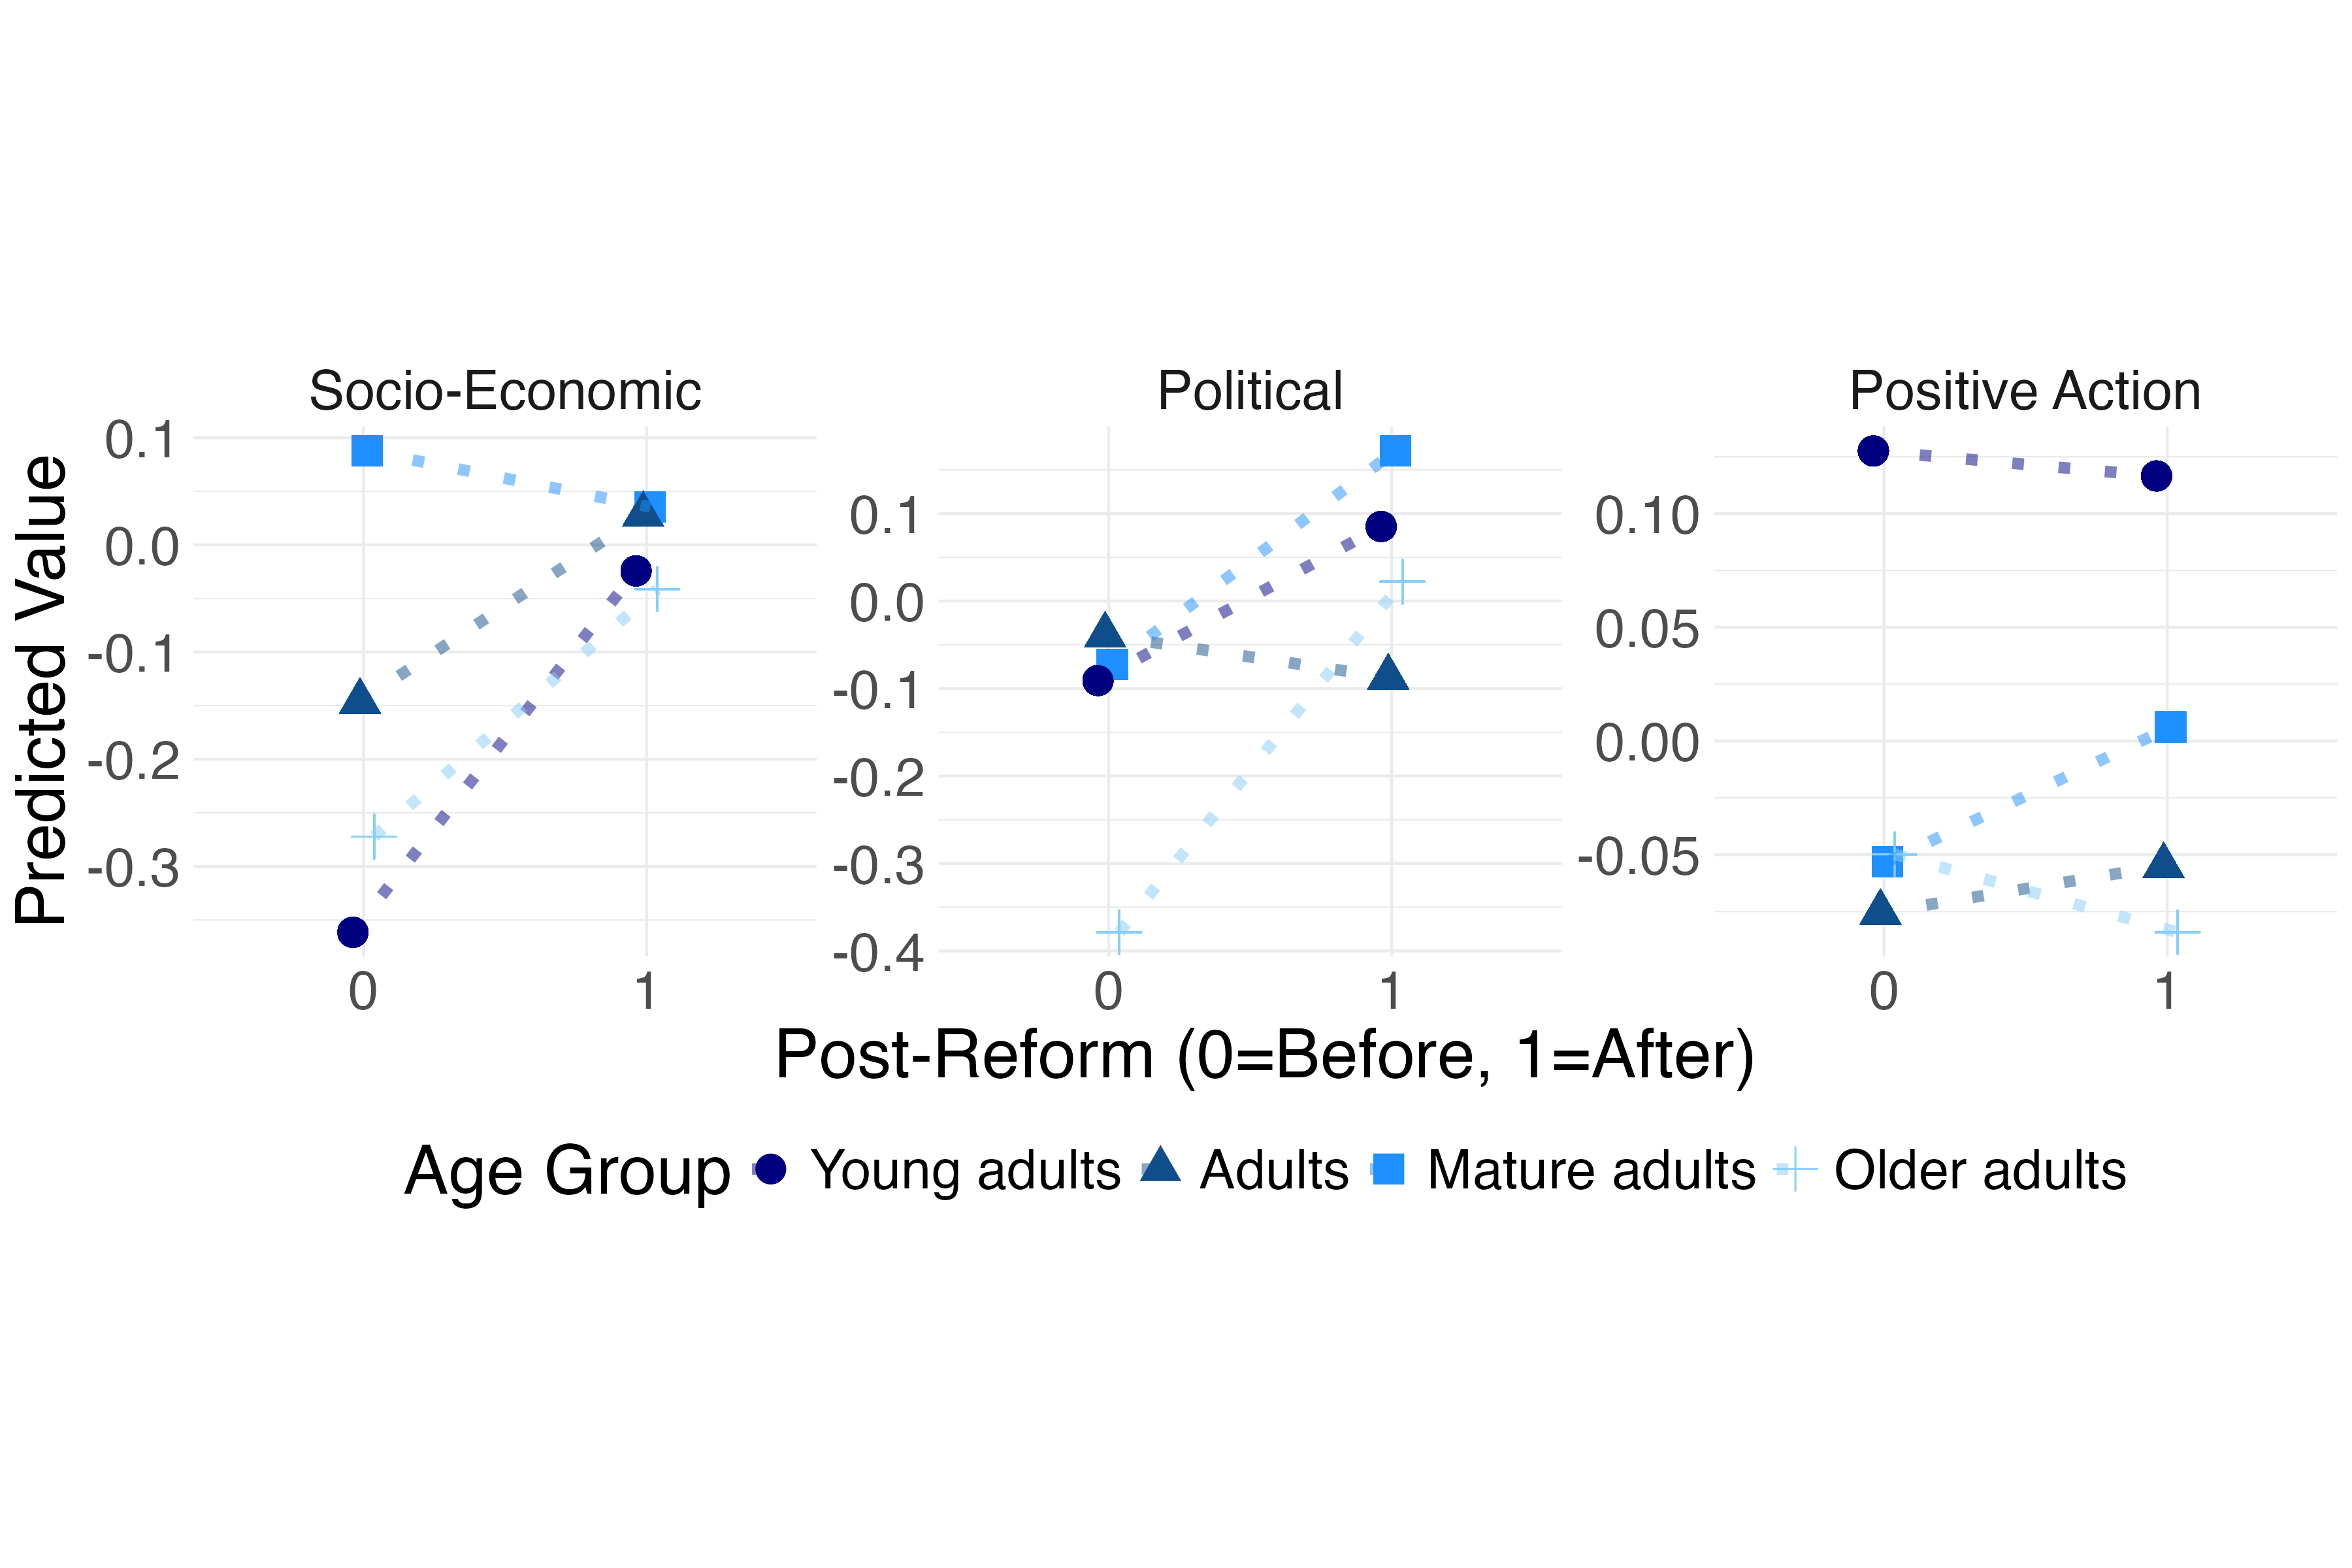
\includegraphics[width=0.9\textwidth]{age_plot}
		\label{fig:age_plot}
	\end{figure}
	
\begin{table}[H]
	\centering
	\caption{Age Models}
	\label{tab:age_models}
	\begin{tabular}{@{\extracolsep{5pt}}p{2.5cm}ccc}
		\hline \hline
		\\[-1.8ex]
		& \multicolumn{3}{c}{\textit{Dependent variable:}} \\
		\cline{2-4}
		\\[-1.8ex]
		& SocEconScale & PolScale & PosActScale \\
		\\[-1.8ex]
		& (1) & (2) & (3)\\
		\hline
		\\[-1.8ex]
		postReform1 & 0.337$^{**}$ & 0.176 & $-$0.011 \\
		& (0.158) & (0.163) & (0.154) \\
		\\
		age\_catAdults & 0.215 & 0.052 & $-$0.203 \\
		& (0.171) & (0.176) & (0.167) \\
		\\
		age\_catMature adults & 0.449$^{***}$ & 0.018 & $-$0.181 \\
		& (0.171) & (0.176) & (0.167) \\
		\\
		age\_catOlder adults & 0.089 & $-$0.288 & $-$0.177 \\
		& (0.188) & (0.193) & (0.183) \\
		\\
		postReform1:age\_\\catAdults & $-$0.163 & $-$0.224 & 0.031 \\
		& (0.209) & (0.216) & (0.204) \\
		\\
		postReform1:age\_\\catMature adults & $-$0.390$^{*}$ & 0.068 & 0.070 \\
		& (0.210) & (0.216) & (0.205) \\
		\\
		postReform1:age\_\\catOlder adults & $-$0.106 & 0.225 & $-$0.023 \\
		& (0.228) & (0.235) & (0.222) \\
		\\
		Constant & $-$0.361$^{***}$ & $-$0.091 & 0.128 \\
		& (0.132) & (0.135) & (0.128) \\
		\\
		\hline
		\\[-1.8ex]
		Observations & 800 & 799 & 799 \\
		R$^{2}$ & 0.016 & 0.018 & 0.006 \\
		Adjusted R$^{2}$ & 0.007 & 0.009 & $-$0.003 \\
		Residual Std. Error & 0.994 (df = 792) & 1.022 (df = 791) & 0.968 (df = 791) \\
		F Statistic & 1.820$^{*}$ (df = 7; 792) & 2.044$^{**}$ (df = 7; 791) & 0.707 (df = 7; 791) \\
		\hline
		\hline
		\\[-1.8ex]
		\textit{Note:} & \multicolumn{3}{r}{$^{*}$p$<$0.1; $^{**}$p$<$0.05; $^{***}$p$<$0.01} \\
	\end{tabular}
\end{table}
	
	\newpage
	\item \textbf{City}: 
	
	\noindent Similar to educational attainment, urban populations tend to be more progressive than rural ones, so we would expect the baseline support for gender equality to be higher among urban parents. As for the interaction, urban versus rural settings could also mediate the effectiveness of fathers' leave, with urban areas possibly being more receptive to such policies due to pre-existing progressive attitudes.
	
	\noindent From Figure 7, we can see that baseline support would seem higher for people in urban environments (except for the Positive Action Scale), while the magnitude of the effect by group changes according to the scale. As Table 5 shows, however, no City or City and Reform interaction coefficients resulted statistically significant. Thus, there is no evidence that rural vs. urban environments cause different levels of support for gender equality or that they mediate the effect of the reform in this case. 
	
	\begin{figure}[H]
		\centering
		\caption{Predicted Effects of Reform with added living in City Variable and Interaction Across Scales}
		\vspace{-1cm}
		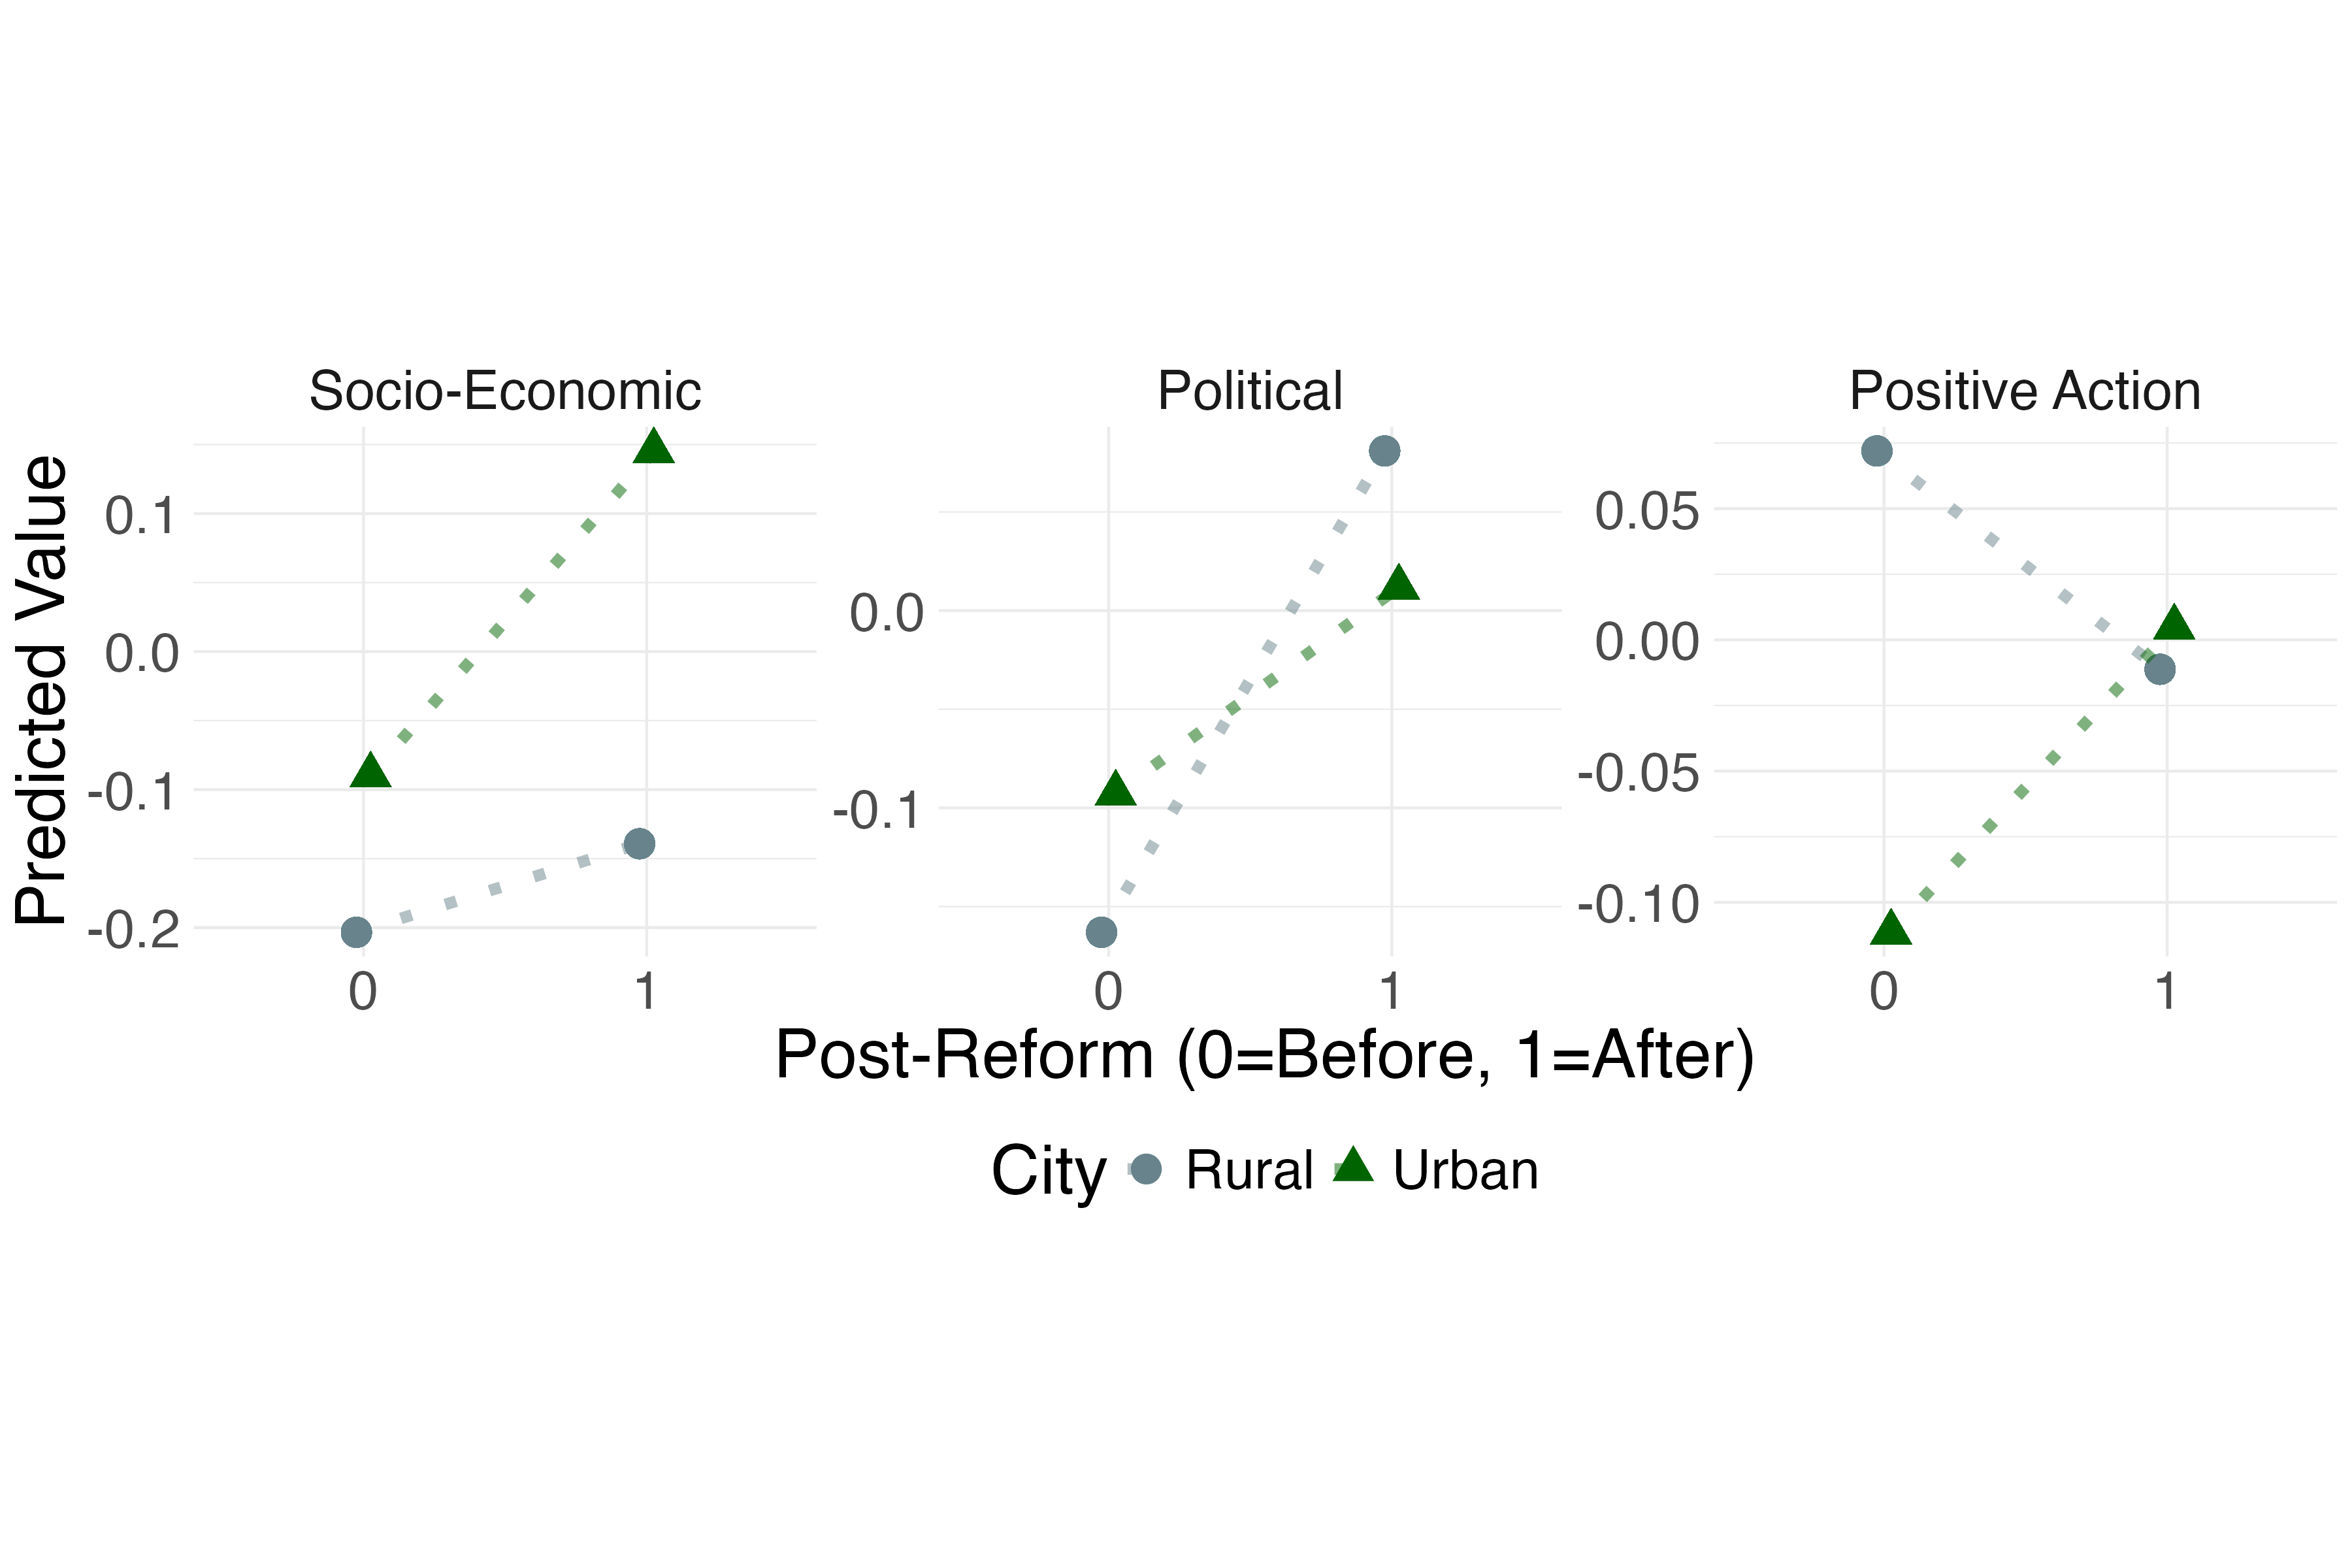
\includegraphics[width=0.9\textwidth]{city_plot}
		\label{fig:city_plot}
	\end{figure}
	
	\begin{table}[H] \centering   \caption{City Models}   \label{} \begin{tabular}{@{\extracolsep{5pt}}lccc} \\[-1.8ex]\hline \hline \\[-1.8ex]  & \multicolumn{3}{c}{\textit{Dependent variable:}} \\ \cline{2-4} \\[-1.8ex] & SocEconScale & PolScale & PosActScale \\ \\[-1.8ex] & (1) & (2) & (3)\\ \hline \\[-1.8ex]  postReform1 & 0.064 & 0.244$^{**}$ & $-$0.083 \\   & (0.105) & (0.108) & (0.102) \\   & & & \\  city & 0.114 & 0.070 & $-$0.183 \\   & (0.119) & (0.123) & (0.116) \\   & & & \\  postReform1:city & 0.171 & $-$0.140 & 0.199 \\   & (0.147) & (0.152) & (0.144) \\   & & & \\  Constant & $-$0.203$^{**}$ & $-$0.163$^{*}$ & 0.072 \\   & (0.085) & (0.088) & (0.083) \\   & & & \\ \hline \\[-1.8ex] Observations & 800 & 799 & 799 \\ R$^{2}$ & 0.019 & 0.008 & 0.003 \\ Adjusted R$^{2}$ & 0.016 & 0.004 & $-$0.001 \\ Residual Std. Error & 0.989 (df = 796) & 1.025 (df = 795) & 0.967 (df = 795) \\ F Statistic & 5.267$^{***}$ (df = 3; 796) & 2.037 (df = 3; 795) & 0.861 (df = 3; 795) \\ \hline \hline \\[-1.8ex] \textit{Note:}  & \multicolumn{3}{r}{$^{*}$p$<$0.1; $^{**}$p$<$0.05; $^{***}$p$<$0.01} \\ \end{tabular} \end{table} 
	
	\newpage
	\item \textbf{Children}: 
	
	\noindent The addition of the number of children variable and its interaction with the reform is interesting because previous children might affect the perceived necessity of taking fathers' leave for both parents, which may have implications for its impact on changing gender role attitudes.
	
	\noindent As seen in Figure 8, 
	
	\begin{figure}[H]
		\centering
		\caption{Predicted Effects of Reform with added Number of Children variable and Interaction Across Scales}
		\vspace{-1cm}
		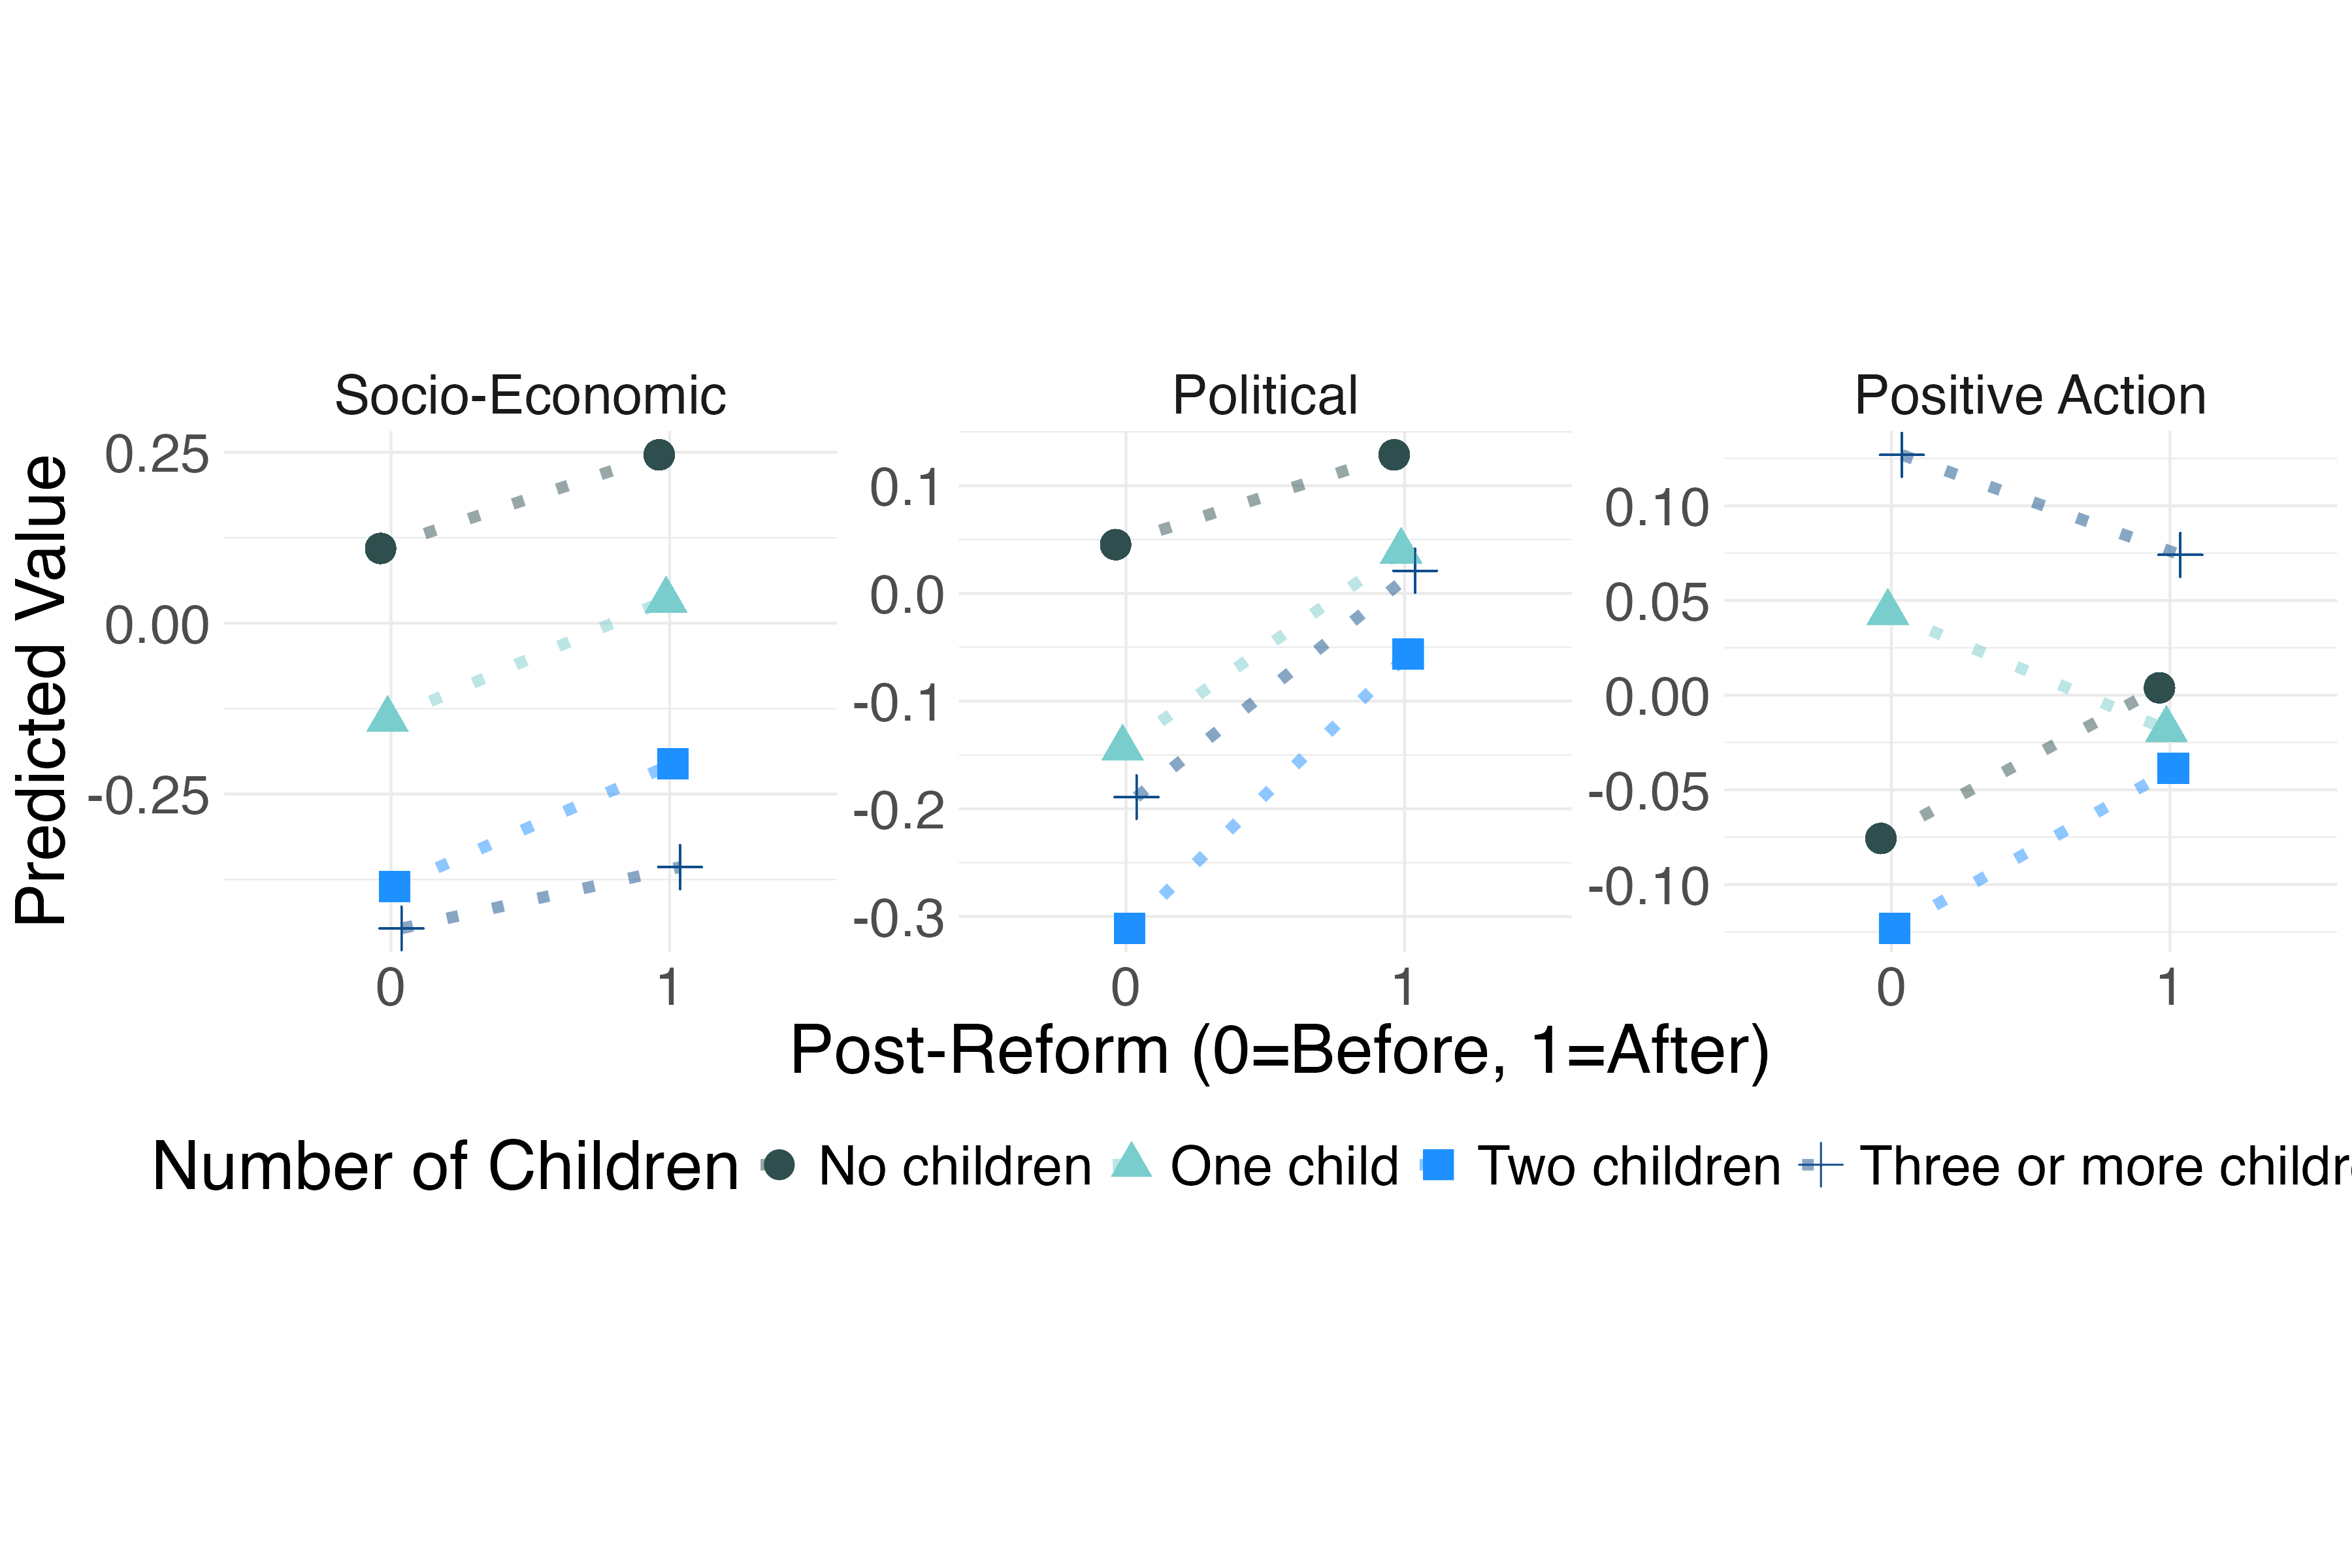
\includegraphics[width=0.9\textwidth]{children_plot}
		\label{fig:children_plot}
	\end{figure}
	
\begin{table}[H] 
	\centering   
	\caption{Children Models}   
	\label{} 
	\begin{tabular}{@{\extracolsep{5pt}}p{10cm}ccc} 
		\hline 
		\hline 
		& \multicolumn{3}{c}{\textit{Dependent variable:}} \\ 
		\cline{2-4} 
		& SocEcon & Pol & PosAct \\ 
		\hline 
		postReform1 & 0.137 & 0.083 & 0.080 \\   
		& (0.131) & (0.137) & (0.130) \\   
		children\_cat &  &  &  \\ 
		One child & -0.250$^{*}$ & -0.189 & 0.119 \\   
		& (0.142) & (0.149) & (0.141) \\  
		Two children & -0.495$^{***}$ & -0.356$^{**}$ & -0.047 \\   
		& (0.164) & (0.172) & (0.164) \\  
		Three or more children & -0.556$^{**}$ & -0.234 & 0.203 \\   
		& (0.226) & (0.237) & (0.225) \\ 
		postReform1: &  &  &  \\
		One child & 0.038 & 0.099 & -0.141 \\   
		& (0.176) & (0.185) & (0.175) \\  
		Two children & 0.043 & 0.171 & 0.005 \\   
		& (0.206) & (0.216) & (0.205) \\  
		Three or more children & -0.047 & 0.127 & -0.132 \\   
		& (0.266) & (0.279) & (0.264) \\  
		Constant & 0.109 & 0.045 & -0.076 \\   
		& (0.107) & (0.112) & (0.106) \\ 
		\hline 
		Observations & 798 & 797 & 797 \\ 
		R$^{2}$ & 0.049 & 0.015 & 0.003 \\ 
		\hline 
		\hline 
	\end{tabular} 
	\begin{flushleft}
		\textit{Note:} $^{*}$p$<$0.1; $^{**}$p$<$0.05; $^{***}$p$<$0.01
	\end{flushleft}
\end{table} 

	\newpage
	\item \textbf{Married}: 
	
	\noindent Marital status could also influence both baseline attitudes and the effects of the reforms on the different Scales. For instance, single parents could have higher baseline support for equality. Regarding the interaction, single parents would also face different considerations and pressures, so perhaps the leave would also affect their views differently. 
		
	\noindent As Figure 9 shows, there is no statistically significant association between marital status, or it's interaction with the reform in any of the scales. The coefficient for marriage alone is significant to the lowest level (p < 0.1) for Positive Action, but given all the previous results this is likely just due to chance. 
	
	\begin{figure}[H]
		\centering
		\caption{Predicted Effects of Reform with added Married variable and Interaction Across Scales}
		\vspace{-1cm}
		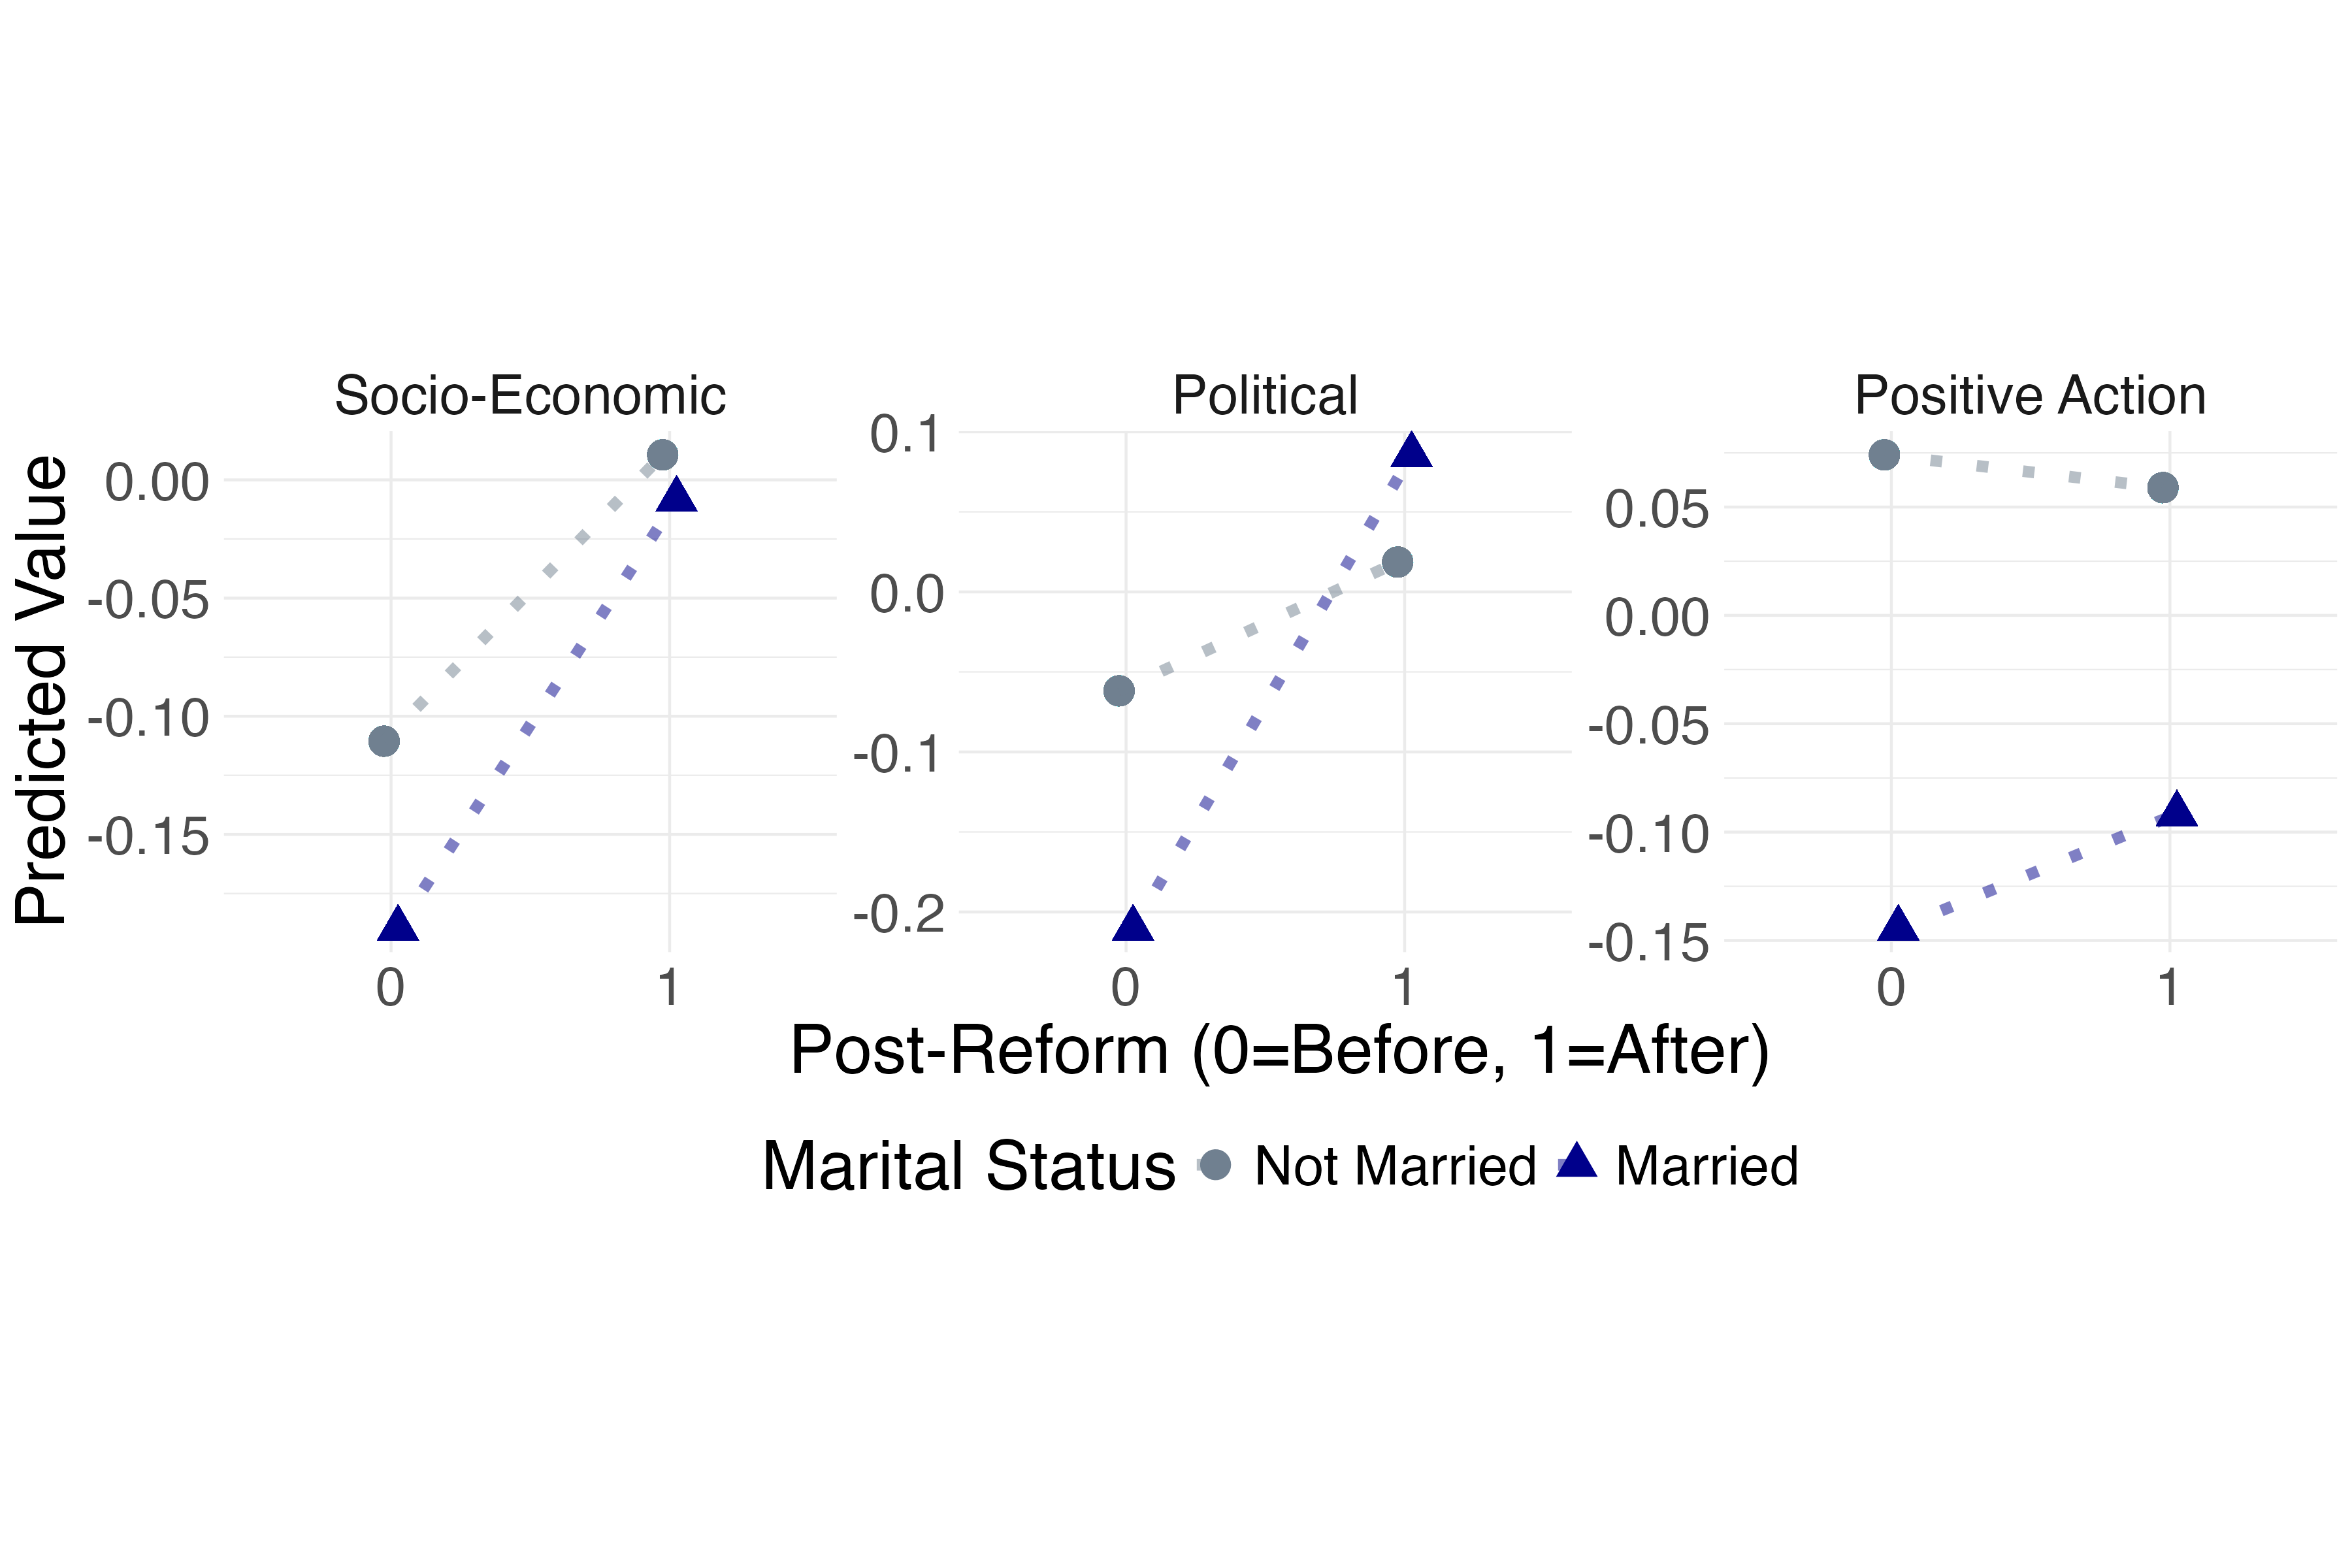
\includegraphics[width=0.9\textwidth]{married_plot}
		\label{fig:married_plot}
	\end{figure}
	
	\begin{table}[H] \centering   \caption{Married Models}   \label{} \begin{tabular}{@{\extracolsep{5pt}}lccc} \\[-1.8ex]\hline \hline \\[-1.8ex]  & \multicolumn{3}{c}{\textit{Dependent variable:}} \\ \cline{2-4} \\[-1.8ex] & SocEconScale & PolScale & PosActScale \\ \\[-1.8ex] & (1) & (2) & (3)\\ \hline \\[-1.8ex]  postReform1 & 0.121 & 0.080 & $-$0.015 \\   & (0.098) & (0.101) & (0.095) \\   & & & \\  married & $-$0.079 & $-$0.148 & $-$0.219$^{*}$ \\   & (0.121) & (0.124) & (0.117) \\   & & & \\  postReform1:married & 0.060 & 0.215 & 0.068 \\   & (0.150) & (0.154) & (0.145) \\   & & & \\  Constant & $-$0.111 & $-$0.062 & 0.074 \\   & (0.080) & (0.082) & (0.077) \\   & & & \\ \hline \\[-1.8ex] Observations & 800 & 799 & 799 \\ R$^{2}$ & 0.006 & 0.009 & 0.008 \\ Adjusted R$^{2}$ & 0.002 & 0.005 & 0.005 \\ Residual Std. Error & 0.996 (df = 796) & 1.024 (df = 795) & 0.964 (df = 795) \\ F Statistic & 1.495 (df = 3; 796) & 2.391$^{*}$ (df = 3; 795) & 2.214$^{*}$ (df = 3; 795) \\ \hline \hline \\[-1.8ex] \textit{Note:}  & \multicolumn{3}{r}{$^{*}$p$<$0.1; $^{**}$p$<$0.05; $^{***}$p$<$0.01} \\ \end{tabular} \end{table} 
	
	\newpage
	\item \textbf{Russian}: 
	
	\noindent Finally, Russian language could be a proxy for cultural background, and perhaps this affects baseline support for gender equality and varying effects of the policy across cultural groups would be expected, with more traditional backgrounds experiencing more significant shifts. Figure 10 shows that both these hypotheses would be the case, as the slopes for Russian speakers (the more conservative background) are steeper and baseline Scale values are higher for non-Russian speakers. However, Table 8 reveals that the coefficients for Russian alone are statistically significant (except for the Positive Action Scale, consistent with all the previous findings), while the estimates for the interaction terms coefficients are not. Thus, there is no evidence for an interactive effect, but there is for an additive one of Russian. 
	
	\begin{figure}[H]
		\centering
		\caption{Predicted Effects of Reform with added Russian Language variable and Interaction Across Scales}
		\vspace{-1cm}
		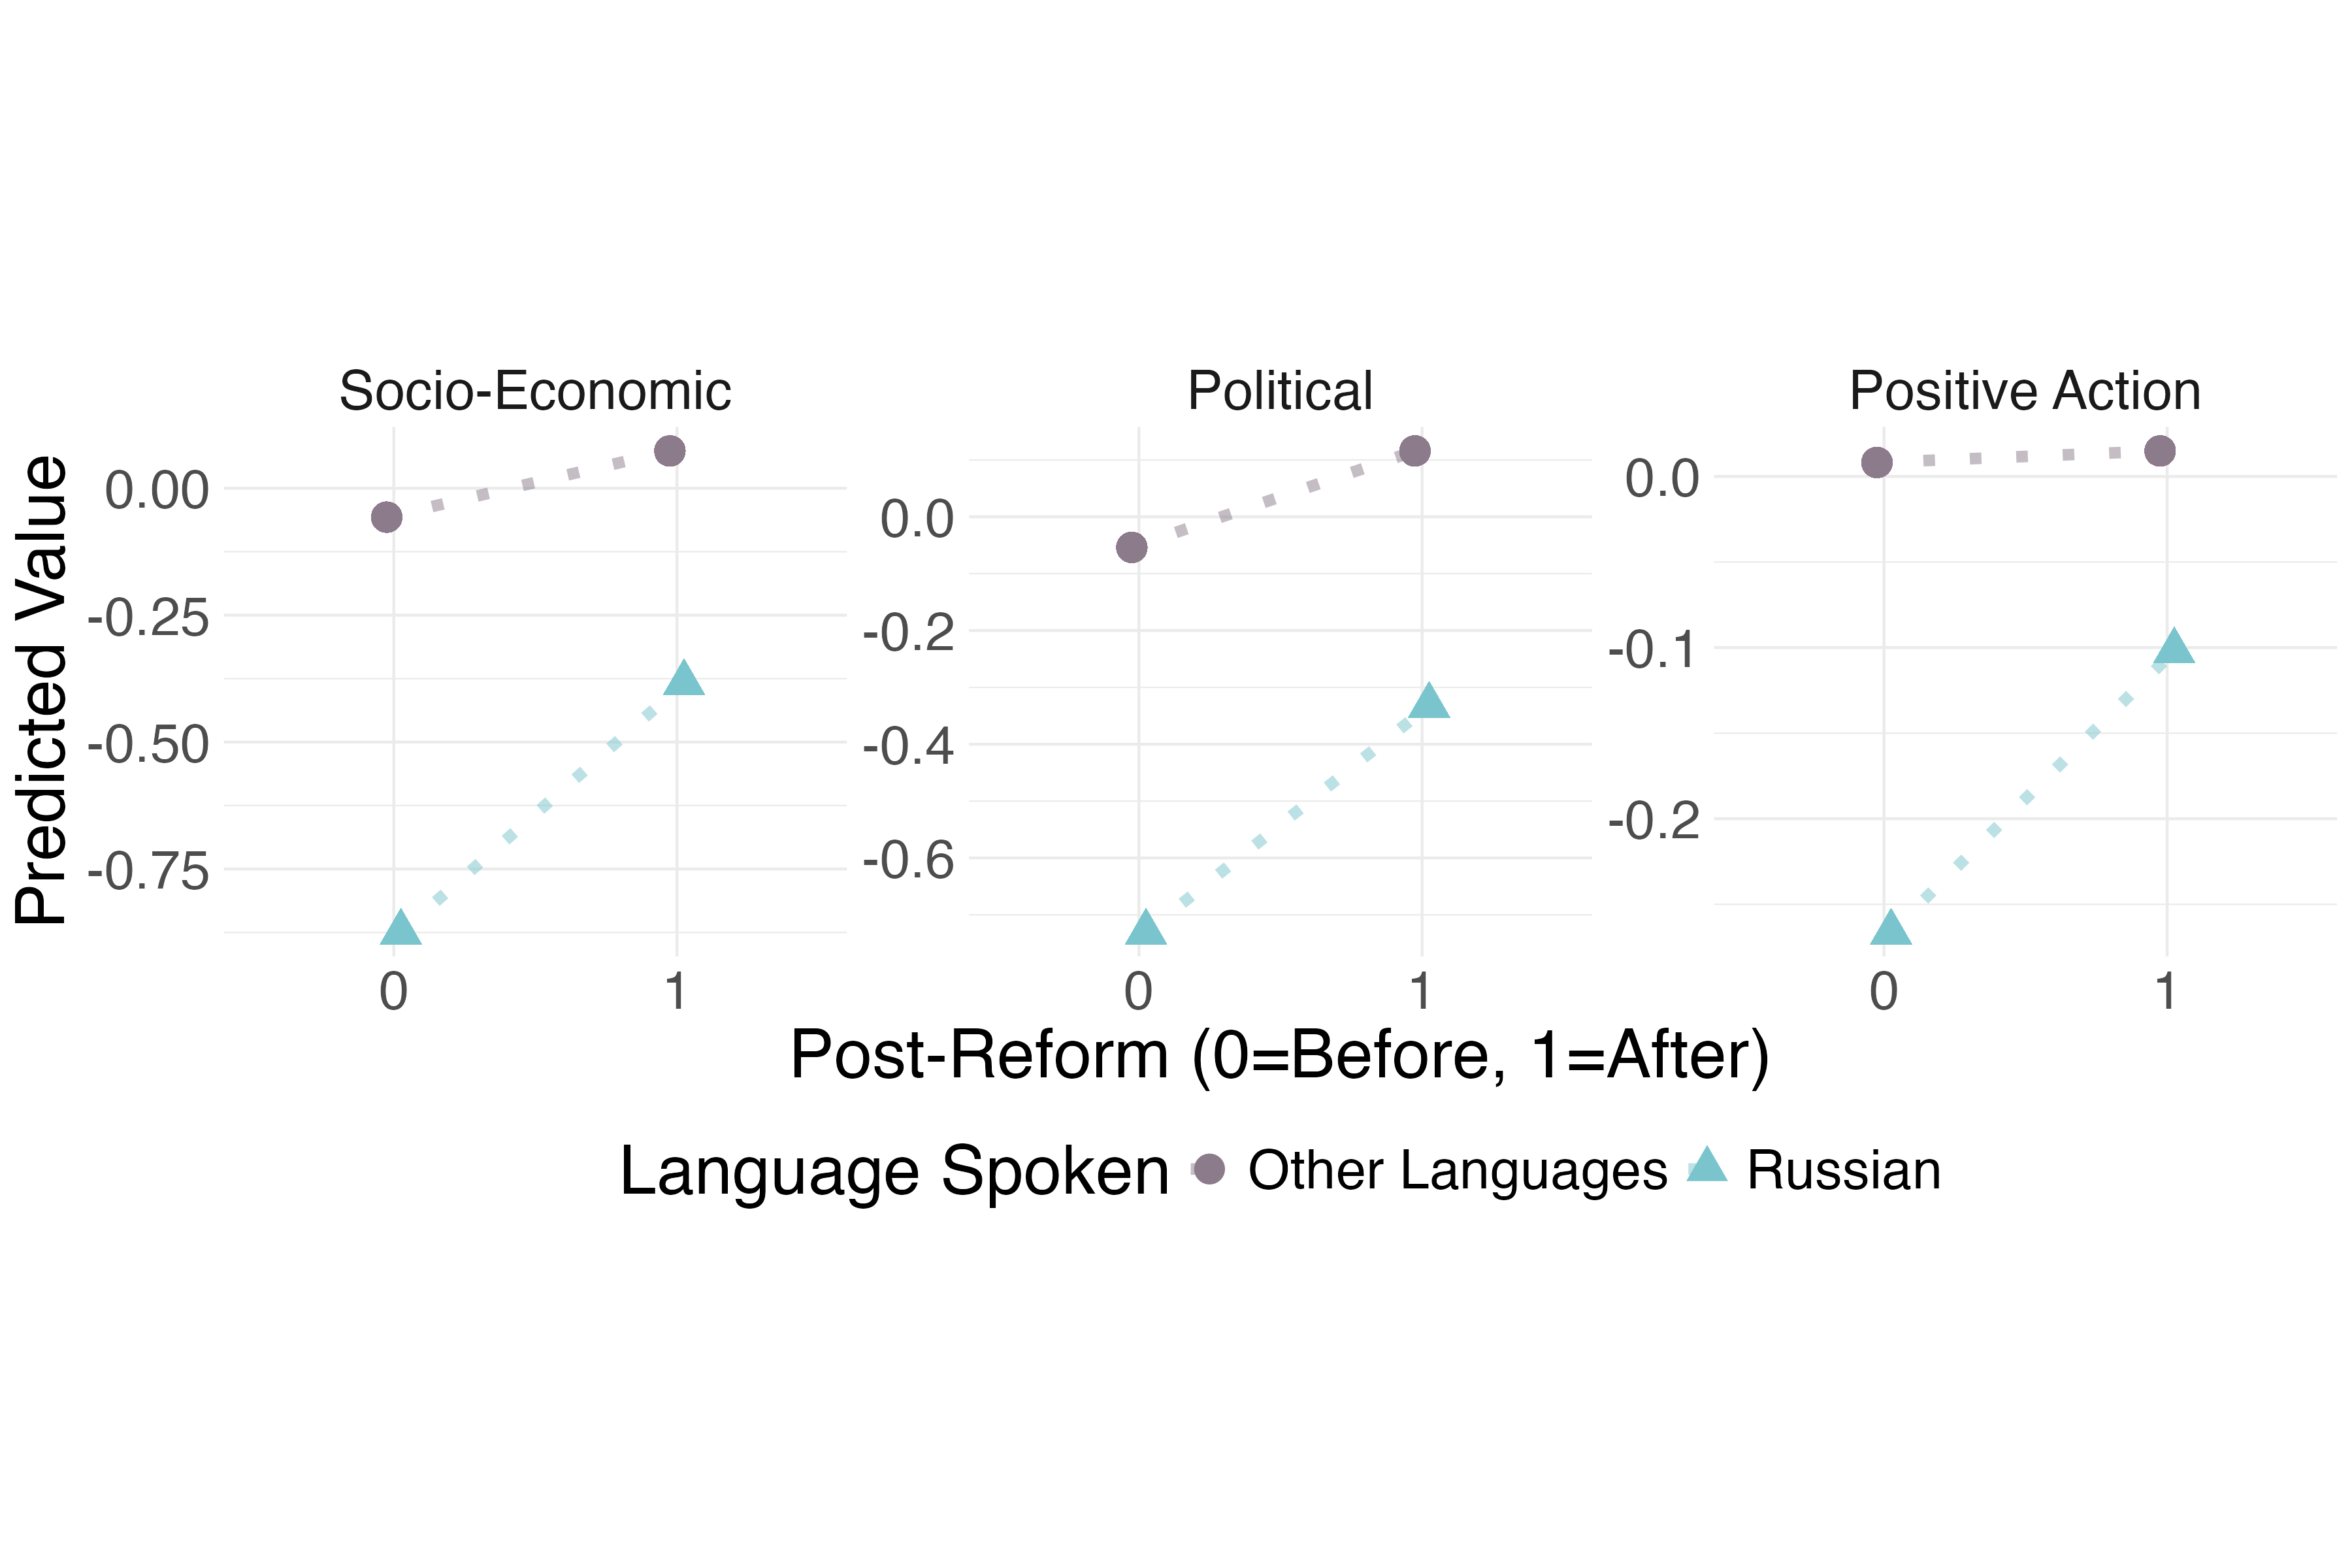
\includegraphics[width=0.9\textwidth]{russian_plot}
		\label{fig:russian_plot}
	\end{figure}
	
	\begin{table}[H] \centering   \caption{Language Models}   \label{} \begin{tabular}{@{\extracolsep{5pt}}p{3cm}ccc} \\[-1.8ex]\hline \hline \\[-1.8ex]  & \multicolumn{3}{c}{\textit{Dependent variable:}} \\ \cline{2-4} \\[-1.8ex] & SocEconScale & PolScale & PosActScale \\ \\[-1.8ex] & (1) & (2) & (3)\\ \hline \\[-1.8ex]  postReform1 & 0.130$^{*}$ & 0.170$^{**}$ & 0.007 \\   & (0.078) & (0.080) & (0.077) \\   & & & \\  lang\_russ & $-$0.818$^{***}$ & $-$0.677$^{***}$ & $-$0.274 \\   & (0.189) & (0.195) & (0.187) \\   & & & \\  postReform1:lang\_russ & 0.361 & 0.229 & 0.158 \\   & (0.223) & (0.230) & (0.220) \\   & & & \\  Constant & $-$0.057 & $-$0.054 & 0.008 \\   & (0.062) & (0.064) & (0.062) \\   & & & \\ \hline \\[-1.8ex] Observations & 800 & 799 & 799 \\ R$^{2}$ & 0.046 & 0.037 & 0.004 \\ Adjusted R$^{2}$ & 0.042 & 0.034 & 0.0003 \\ Residual Std. Error & 0.976 (df = 796) & 1.009 (df = 795) & 0.967 (df = 795) \\ F Statistic & 12.652$^{***}$ (df = 3; 796) & 10.283$^{***}$ (df = 3; 795) & 1.075 (df = 3; 795) \\ \hline \hline \\[-1.8ex] \textit{Note:}  & \multicolumn{3}{r}{$^{*}$p$<$0.1; $^{**}$p$<$0.05; $^{***}$p$<$0.01} \\ \end{tabular} \end{table} 
	
\end{enumerate}
\newpage
\section*{Conclusions}

\noindent In sum, this paper replicated the tables and figures found in the main text of the article by Tavits, Schleiter, Homola \& Ward, and added to the study by exploring models with added variables and the interaction between such variables and the daddy leave reform. Overall, the results show evidence that some of these variables have statistically significant associations with the outcome Scales, while few such relationships were found for the interactions. Thus, the explored variables better explain the outcomes as controls, rather than as mediators of the effect of the reform. 

\vspace{0.5cm}
\section*{References} 

Tavits, M., Schleiter, P., Homola, J., \& Ward, D. (2024). Fathers’Leave Reduces Sexist Attitudes. American Political Science Review, 118(1), 488–494. doi:10.1017/S0003055423000369

\end{document}
